\documentclass[fleqn]{article}
\oddsidemargin 0.0in
\textwidth 6.0in
\thispagestyle{empty}
\usepackage{import}
\usepackage{amsmath}
\usepackage{graphicx}
\usepackage{flexisym}
\usepackage{calligra}
\usepackage{amssymb}
\usepackage{bigints} 
\usepackage[english]{babel}
\usepackage[utf8x]{inputenc}
\usepackage{float}
\usepackage[colorinlistoftodos]{todonotes}


\DeclareMathAlphabet{\mathcalligra}{T1}{calligra}{m}{n}
\DeclareFontShape{T1}{calligra}{m}{n}{<->s*[2.2]callig15}{}
\newcommand{\scriptr}{\mathcalligra{r}\,}
\newcommand{\boldscriptr}{\pmb{\mathcalligra{r}}\,}

\definecolor{hwColor}{HTML}{AD53BA}

\begin{document}

  \begin{titlepage}

    \newcommand{\HRule}{\rule{\linewidth}{0.5mm}}

    \center

    \begin{center}
      
\includegraphics[height=11cm, width=11cm]{asu.png}
    \end{center}

    \vline

    \textsc{\LARGE Advanced Laboratory I}\\[1.5cm]

    \HRule \\[0.5cm]
    { \huge \bfseries Compton Scattering}\\[0.4cm] 
    \HRule \\[1.0cm]

    \textbf{Behnam Amiri}

    \bigbreak

    \textbf{Prof: Ralph Chamberlin}

    \bigbreak

    \textbf{Lab Partners: Daniel Henningsen, Micah Smith, Srihari Ravi}

    \bigbreak

    \textbf{{\large \today}\\[2cm]}

    \vfill

  \end{titlepage}

  \textbf{Abstract}

  \vspace{10px}

  The Compton scattering process plays significant roles in atomic and molecular physics, condensed matter physics, nuclear physics and material science.
  It could provide useful information on the electromagnetic interaction between light and matter. Several aspects of many-body physics,
  such us electronic structures, electron momentum distributions, many-body interactions of bound electrons, etc., can be revealed by Compton scattering 
  experiments.

  \vspace{30px}

  \textbf{I. Introduction}

  \vspace{10px}

  By $1920$ the successes of the quantum theories of blackbody spectra (Planck, $1901$), the photoelectric effect (Einstein, $1905$) 
  and the hydrogen spectrum (Bohr, $1913$) had established the idea that interactions between electromagnetic radiation of frequency $v$ and matter
  occuer through the emission or absorption of discrete quanta of energy $E=hv$. The next crucial step in the development of the modern concept
  of the photon as the particle of electromagnetic radiation was taken by Arthur Compton in the interpretation 
  of experiments he initiated in $1920$ to measure with precision the wavelengths of X-rays scattered from electrons in materials of 
  (low atomic number). The phenomena of X-ray scattering had already been studied intensively. It was known that the 
  penetrating power of X-rays decreases with increasing wavelength and that X-rays are less penetrating after being scattered than 
  before, which indicated that the scattering process somehow increases their wavelength. 

  Compton’s idea was to use the recently developed 
  technique of high-resolution X-ray spectrometry, based on measurement of the angle of Bragg reflection of X-rays from crystals, 
  to measure precisely the wavelengths of the scattered X-rays. Irradiating a carbon target with an intense collimate beam of monochromatic molybdenum 
  $K_{\alpha}$ X-rays and using an ionization chamber as the detector in his spectrometer, Compton found that the
  spectrum of scattered X-rays had two distinct spectral lines, one at the wavelength of the incident X-rays and another at a wavelength that was 
  longer by an amount that depends on the angle of scattering. The scattering without a wavelength shift was readily explained by the classical theory 
  of coherent scattering of electromagnetic waves from electrons bound in atoms. However, the classical theory provided no explanation of the 
  wavelength-shifting \emph{incoherent} scattering process. The phenomenon of Bragg reflection used in Compton’s measurements was a clear demonstration 
  of the wavelike character of the X-rays. 

  \vspace{30px}

  \textbf{II. Background Information}

  \vspace{10px}

  The Compton scattering or in other words, inelastic scattering of electrons by X-rays is a powerful probe to investigate the behavior of valence 
  electrons in any material. Spectra of Compton scattered photons provides peculiar information about the electron momentum distribution of 
  valence electrons of target materials and hence their electronic properties. If the incident radiation has degree of circular polarization, 
  then the Compton scattering from unpaired electrons, so called magnetic Compton scattering, enables to probe the spin momentum 
  distribution in the ferro- and ferri-magnetic materials.

  \vspace{10px}

  \textbf{III. Theory}

  Albert Einstein postulated that light is \emph{quantized} as photons which can behave like a wave. A photon has energy which corresponds
  to the Plank's energy and momentum which match with the de Broglie's relationship as it is stated with the following equations.
  \\
  \vspace{10px}
  \\
  $E=\hbar \omega ~~~~~~~~~~~~ (1) ~~ \text{(Energy of photon $E$, reduced Planck's constant $\hbar$, angular frequency $\omega$)}$
  \\
  \\
  $p=\hbar k ~~~~~~~~~~~~~ (2) ~~ \text{(momentum $p$, wave vector $k$)}$
  \\
  \\

  Compton demonstrated that photons can behave like particles. Compton conducted an experiment which involved scattering X-ray 
  photons by colliding of photons with electrons as shown in Fig (1).

  \begin{figure}[htbp]
    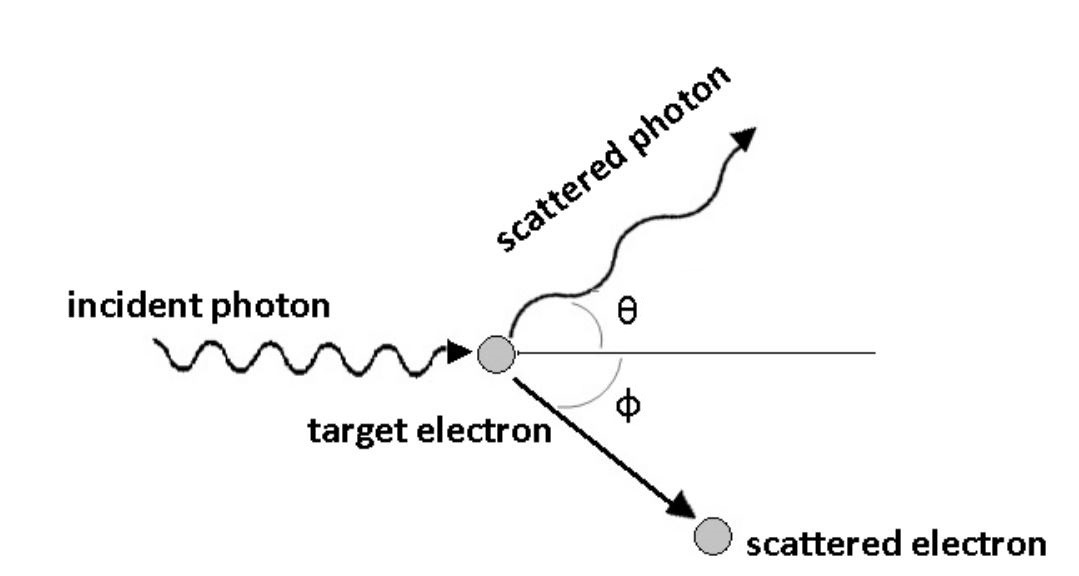
\includegraphics[height=5cm, width=10cm]{One.JPG}
    \caption{
      The incident photon colides with an electron at rest. After the collision the photon transfers some of its energy to the 
      electron. As a result the electron and photon recoil at angle $\phi$ and $\theta$ respectively, known as Compoton Scattering 
    }
  \end{figure}

  \vspace{15px}

  Based on the conservation of energy and momentum and using Eq $(1)$ and Eq $(2)$ we can conclude the following equation which shows
  how the wavelength of the photon changes before and after the collision due the the Compton Effect. For a photon scattered from
  a free electron predict a frequency shift of the photon given by
  $$\Delta \lambda=\dfrac{2 \pi \hbar}{mc} \left[1-cos(\theta)\right]=\lambda_c \left[1-cos(\theta)\right]  ~~~~~~~ (3)$$

  where $\lambda_c \approx 2.4 ~ pm$ is the Compton wavelength, with $m$ the mass of the electron. The corresponding energy shift is given by
  $$\dfrac{E^'}{E}=\dfrac{1}{1+\left(\dfrac{E}{mc^2}\right)\left(1-cos (\theta)\right)} ~~~~~~~ (4)$$

  \vspace{10px}

  \textbf{IV. Experimental Procedure}

  \vspace{10px}

  Todo:(Add description) We just followed the given steps in the lab.


  \begin{figure}[htbp]
    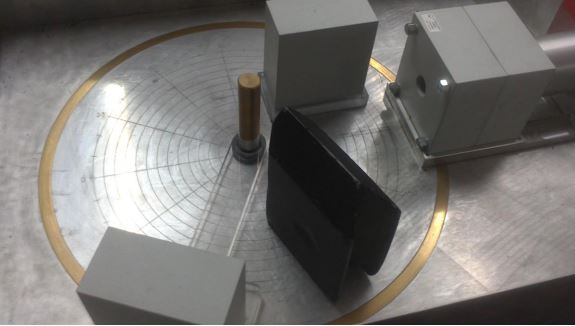
\includegraphics[height=5cm, width=10cm]{Two.JPG}
    \caption{
      Lead blocks were placed between the Cs-137 and the scintillation counter to prevent gamma rays from the
      Cs-137 travelling directly into the scintillation counter without being scattered
    }
  \end{figure}

  \pagebreak

  \textbf{V. Results}

  Todo: Add description....

  \vspace{10px}

  \begin{figure}[htbp]
    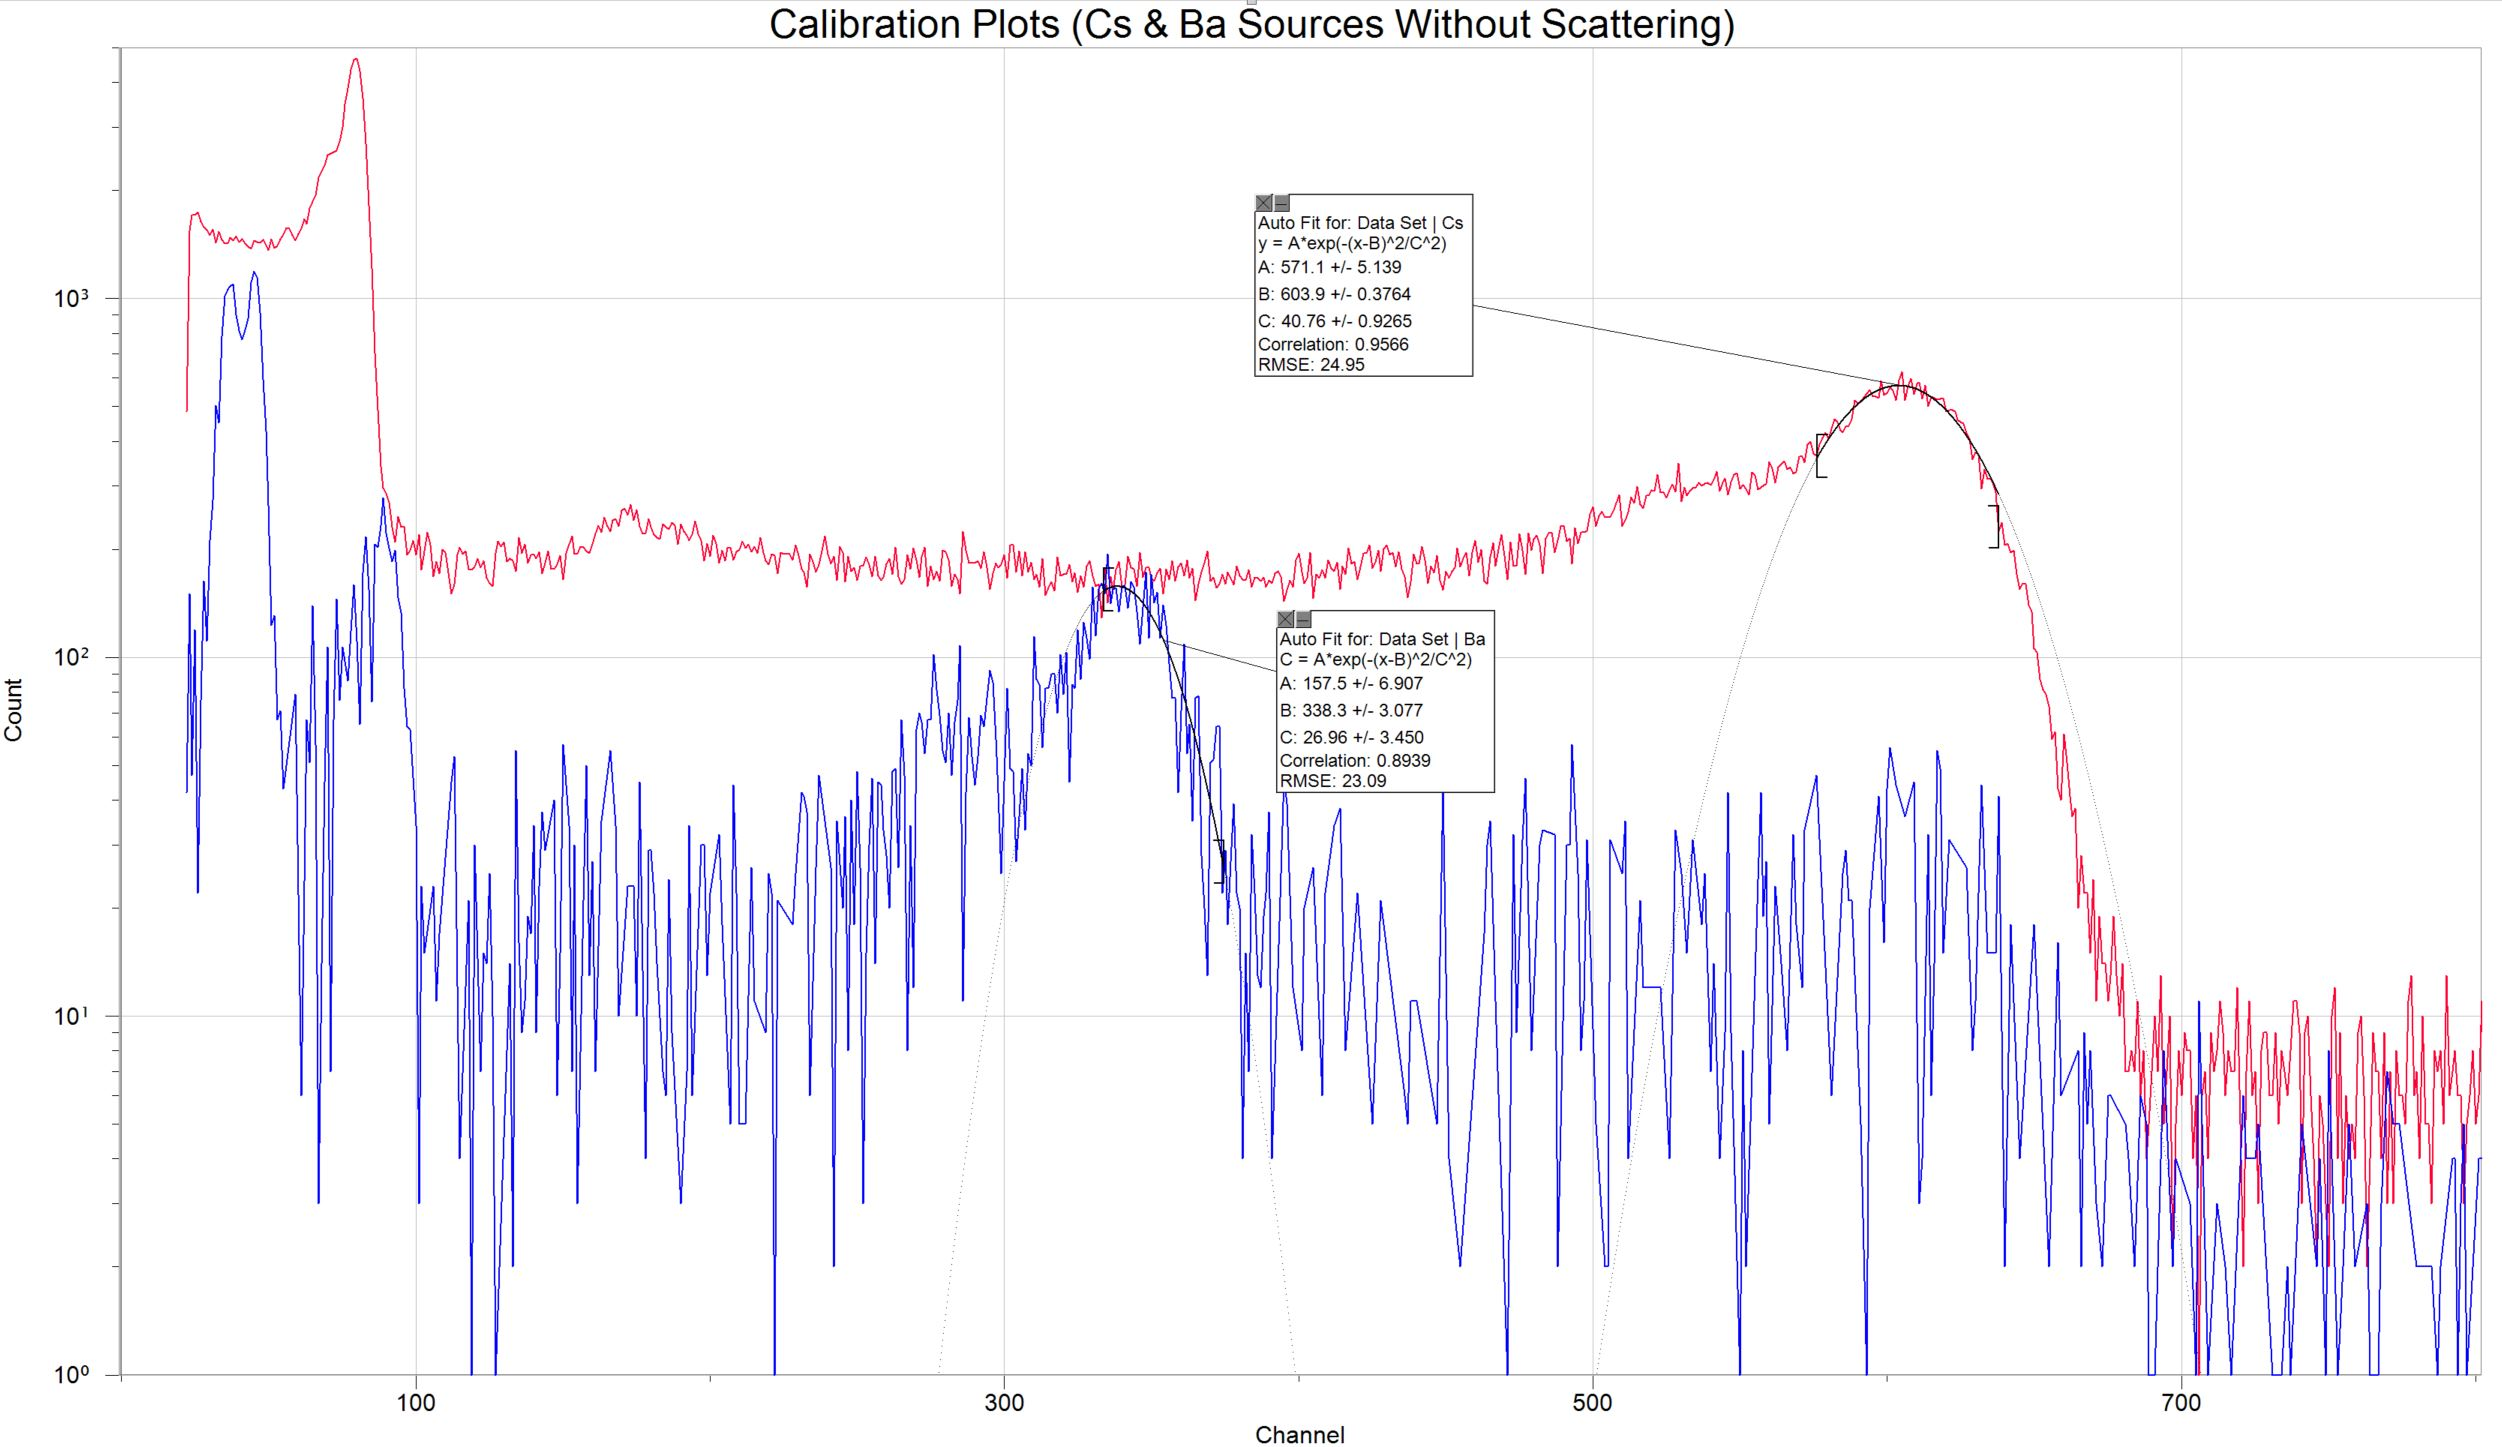
\includegraphics[height=10cm, width=18cm]{Three.JPG}
    \caption{
      Todo
    }
  \end{figure}

  \pagebreak

  \begin{figure}[htbp]
    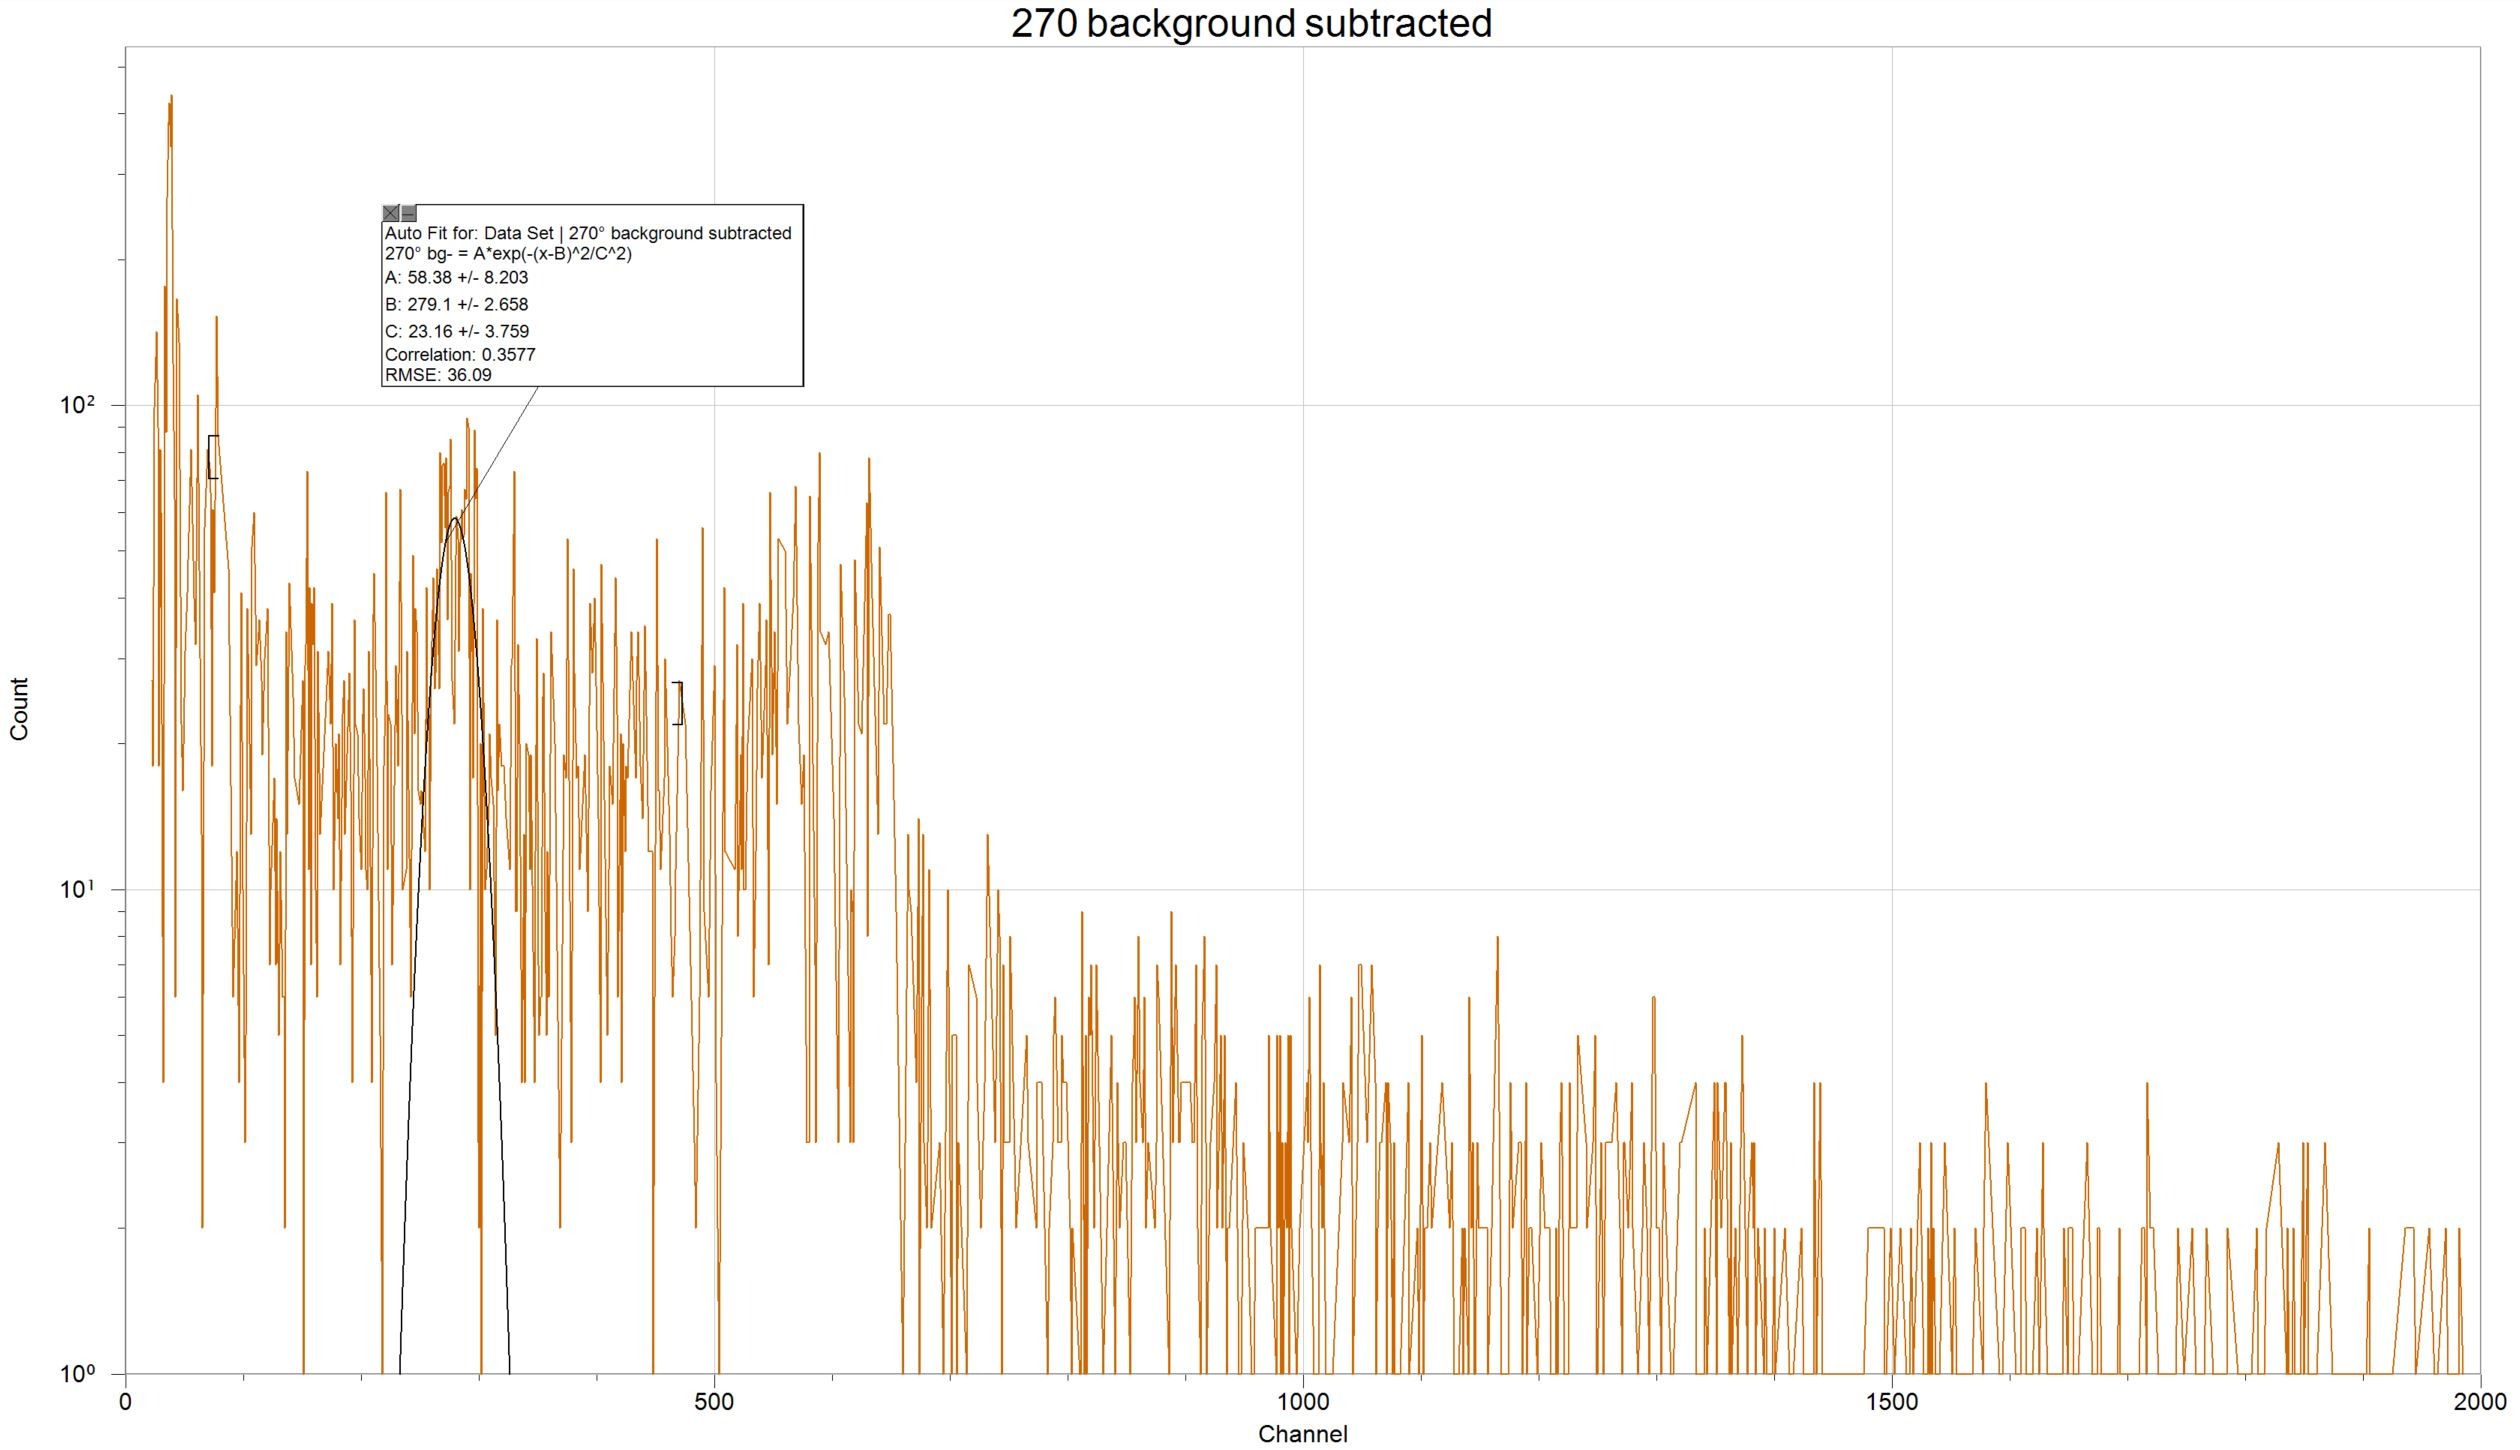
\includegraphics[height=10cm, width=18cm]{Four.JPG}
    \caption{
      Todo
    }
  \end{figure}

  \pagebreak

  \begin{figure}[htbp]
    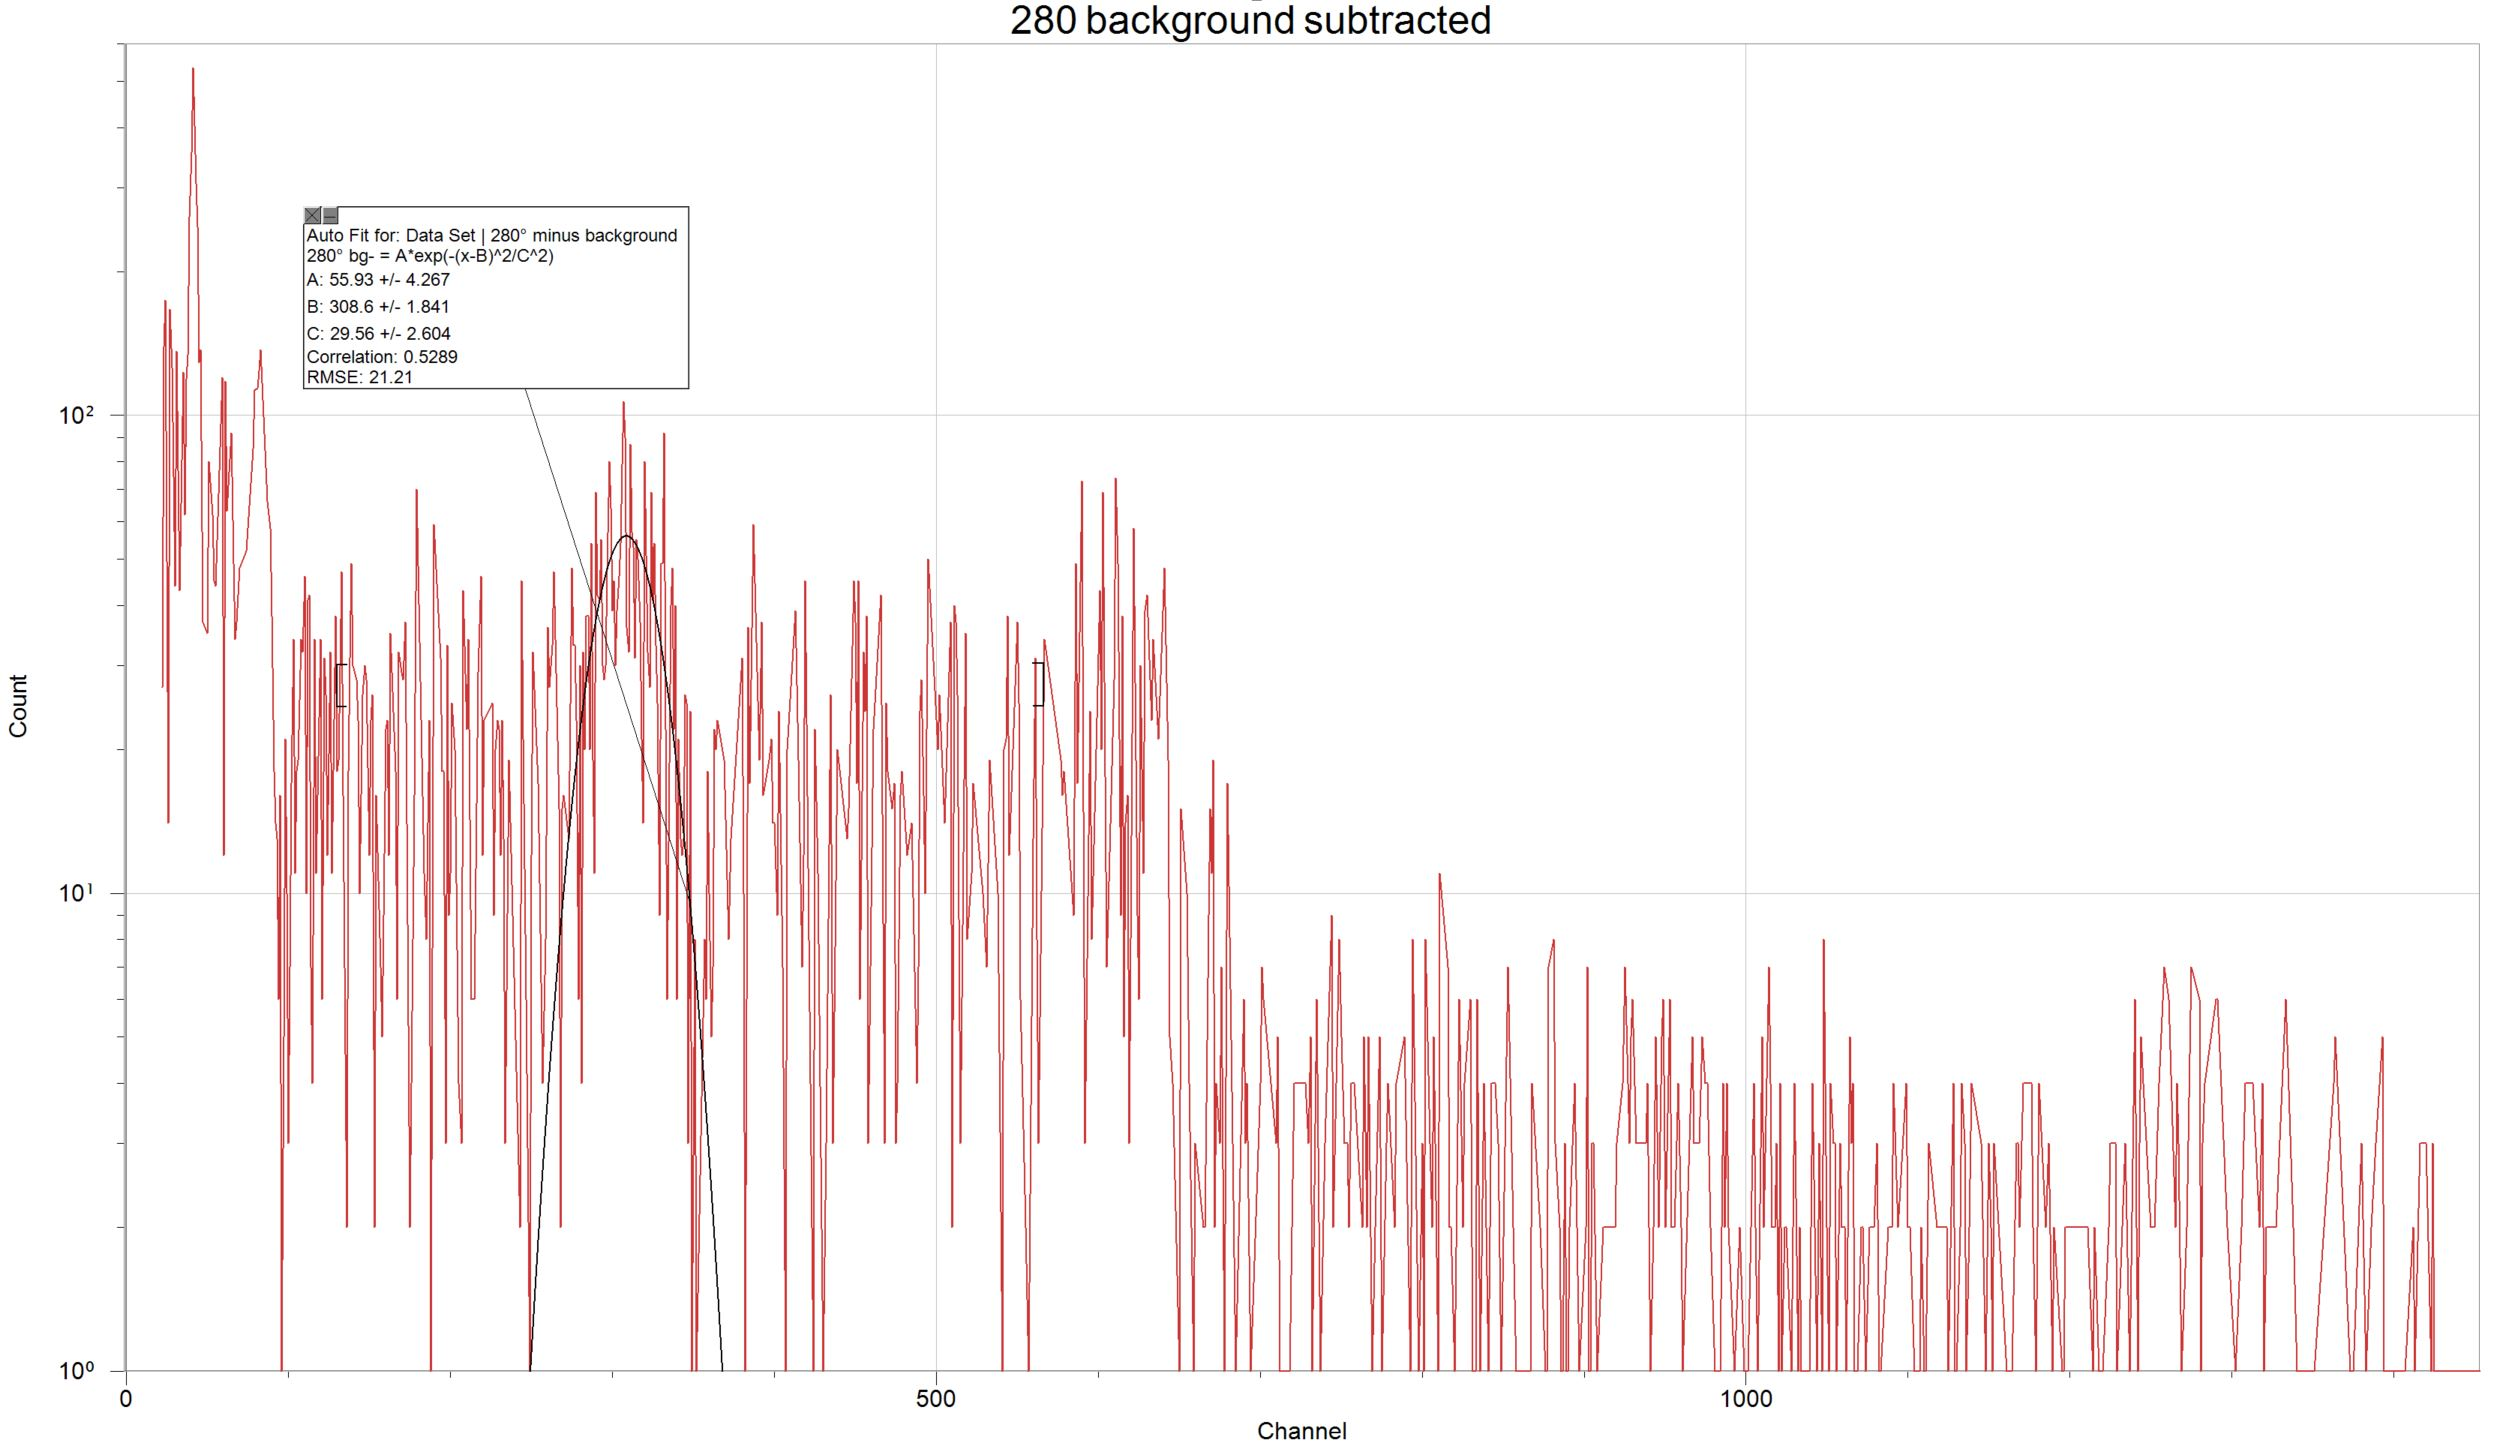
\includegraphics[height=10cm, width=18cm]{Five.JPG}
    \caption{
      Todo
    }
  \end{figure}

  \pagebreak

  \begin{figure}[htbp]
    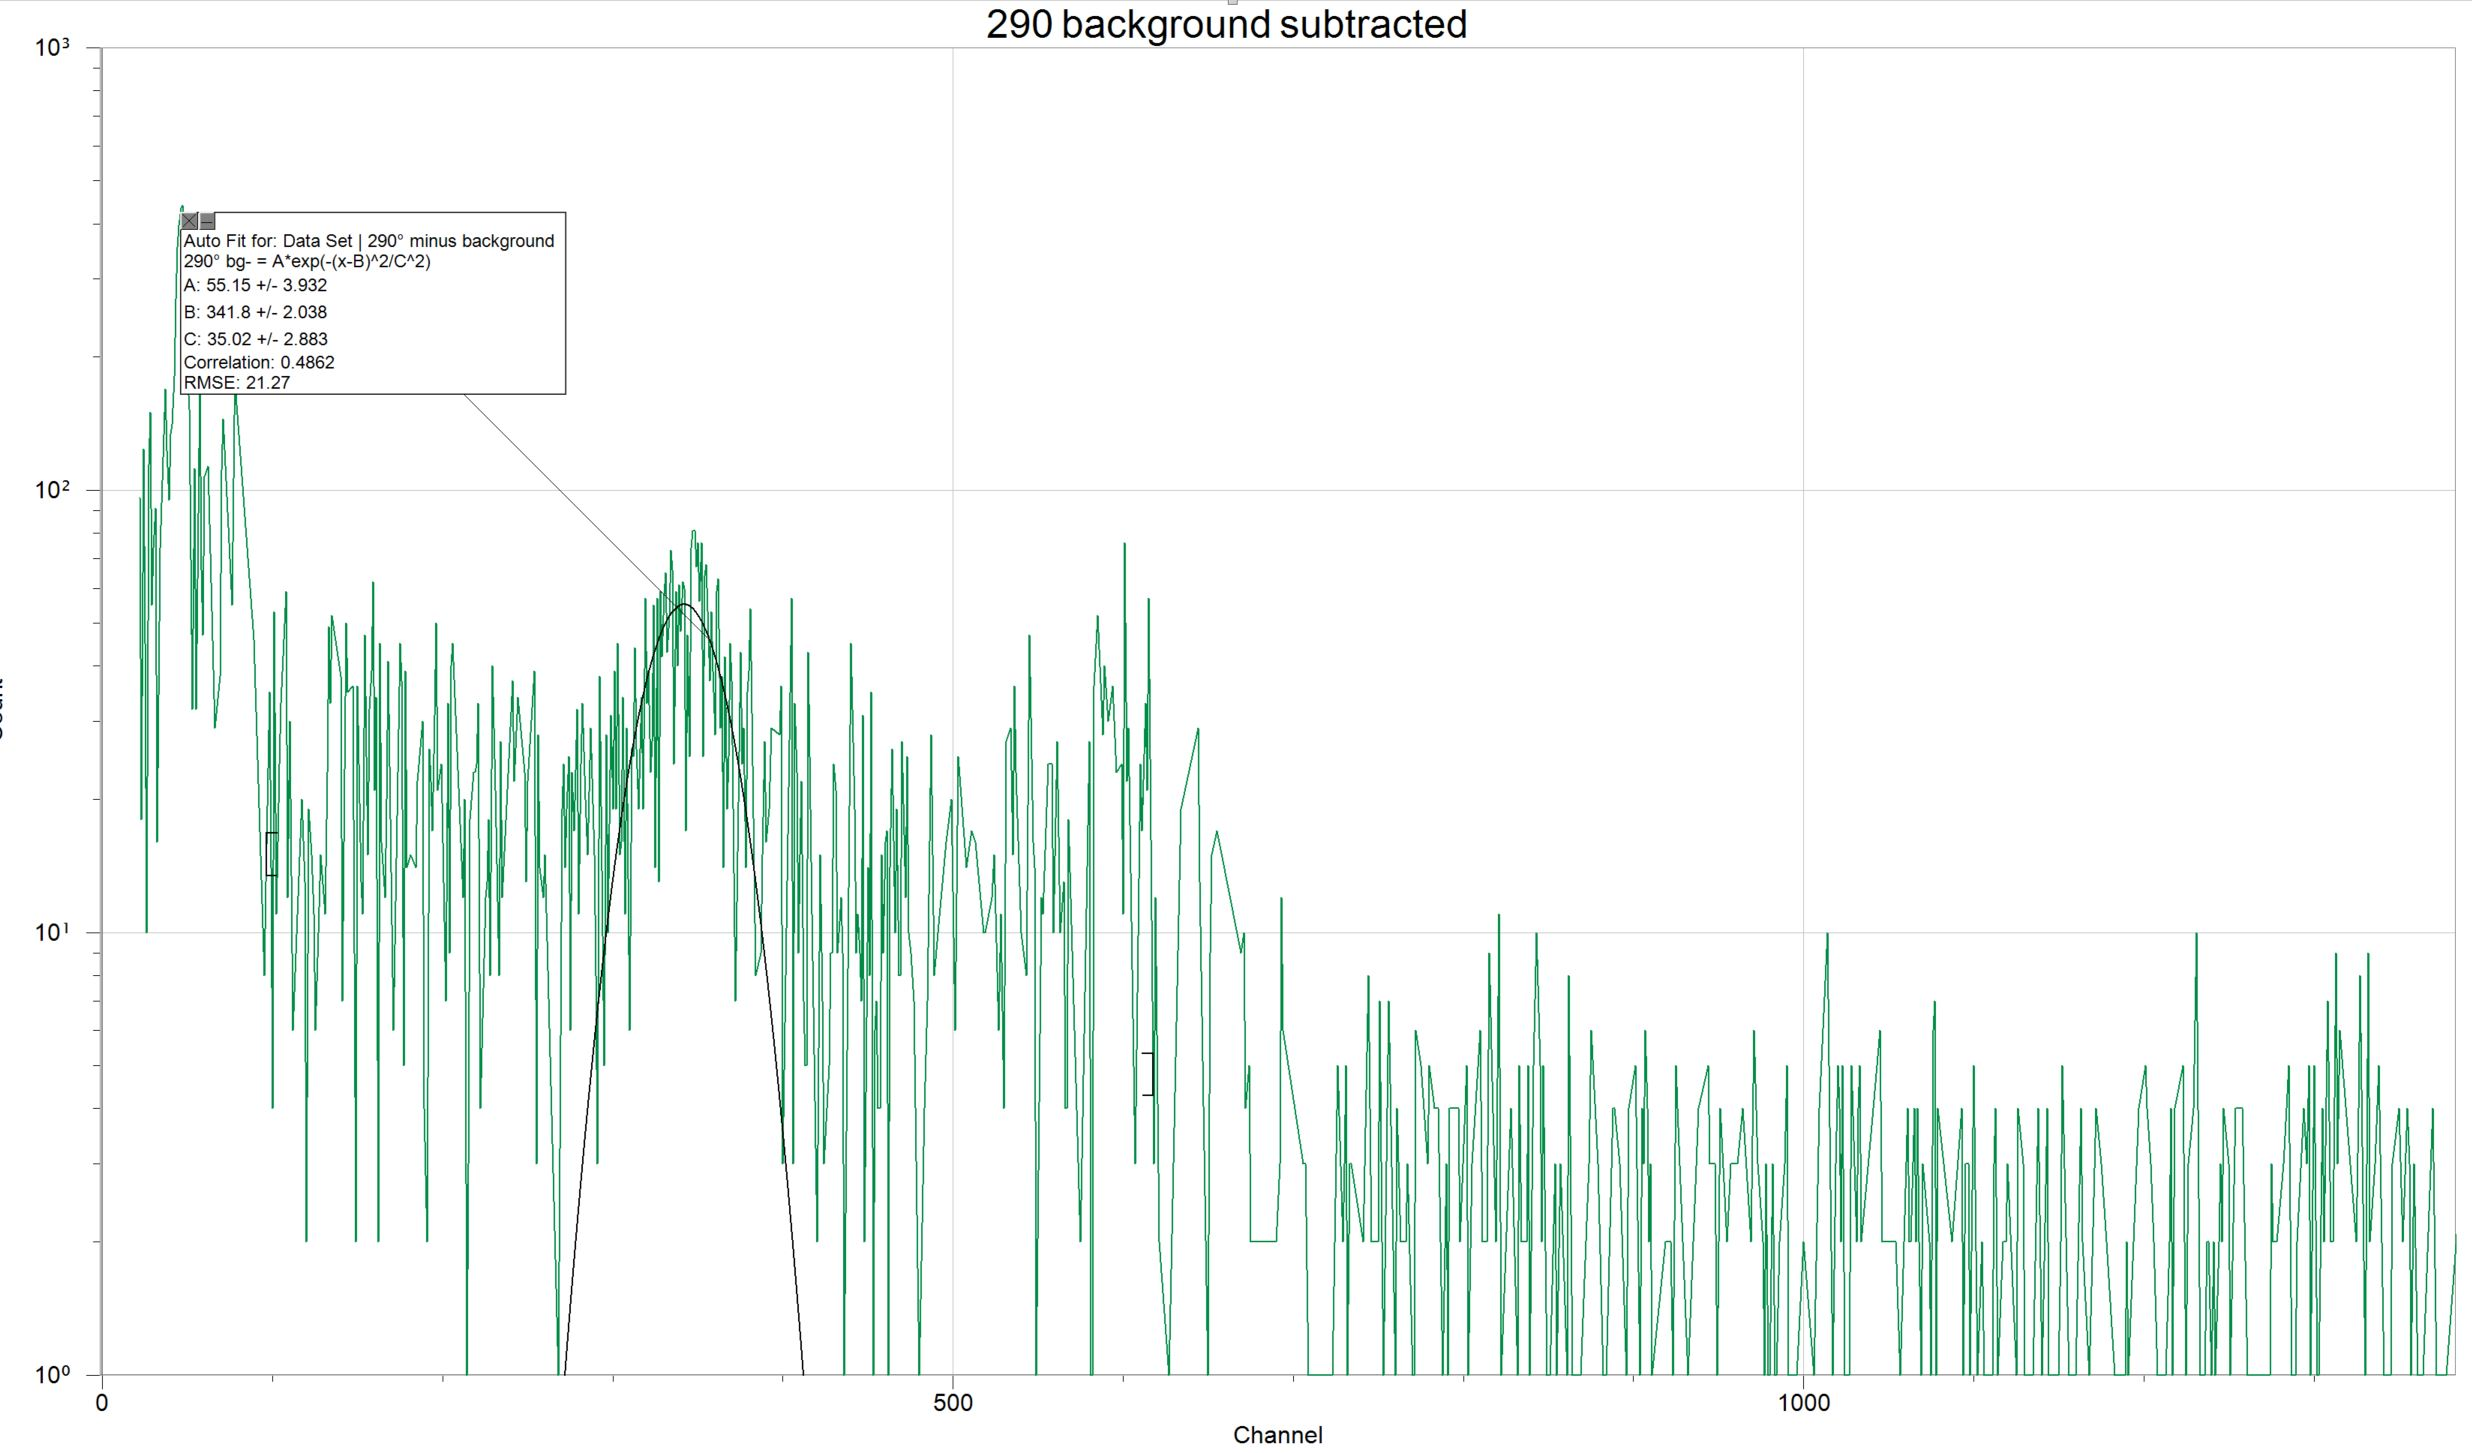
\includegraphics[height=10cm, width=18cm]{Six.JPG}
    \caption{
      Todo
    }
  \end{figure}

  \pagebreak

  \begin{figure}[htbp]
    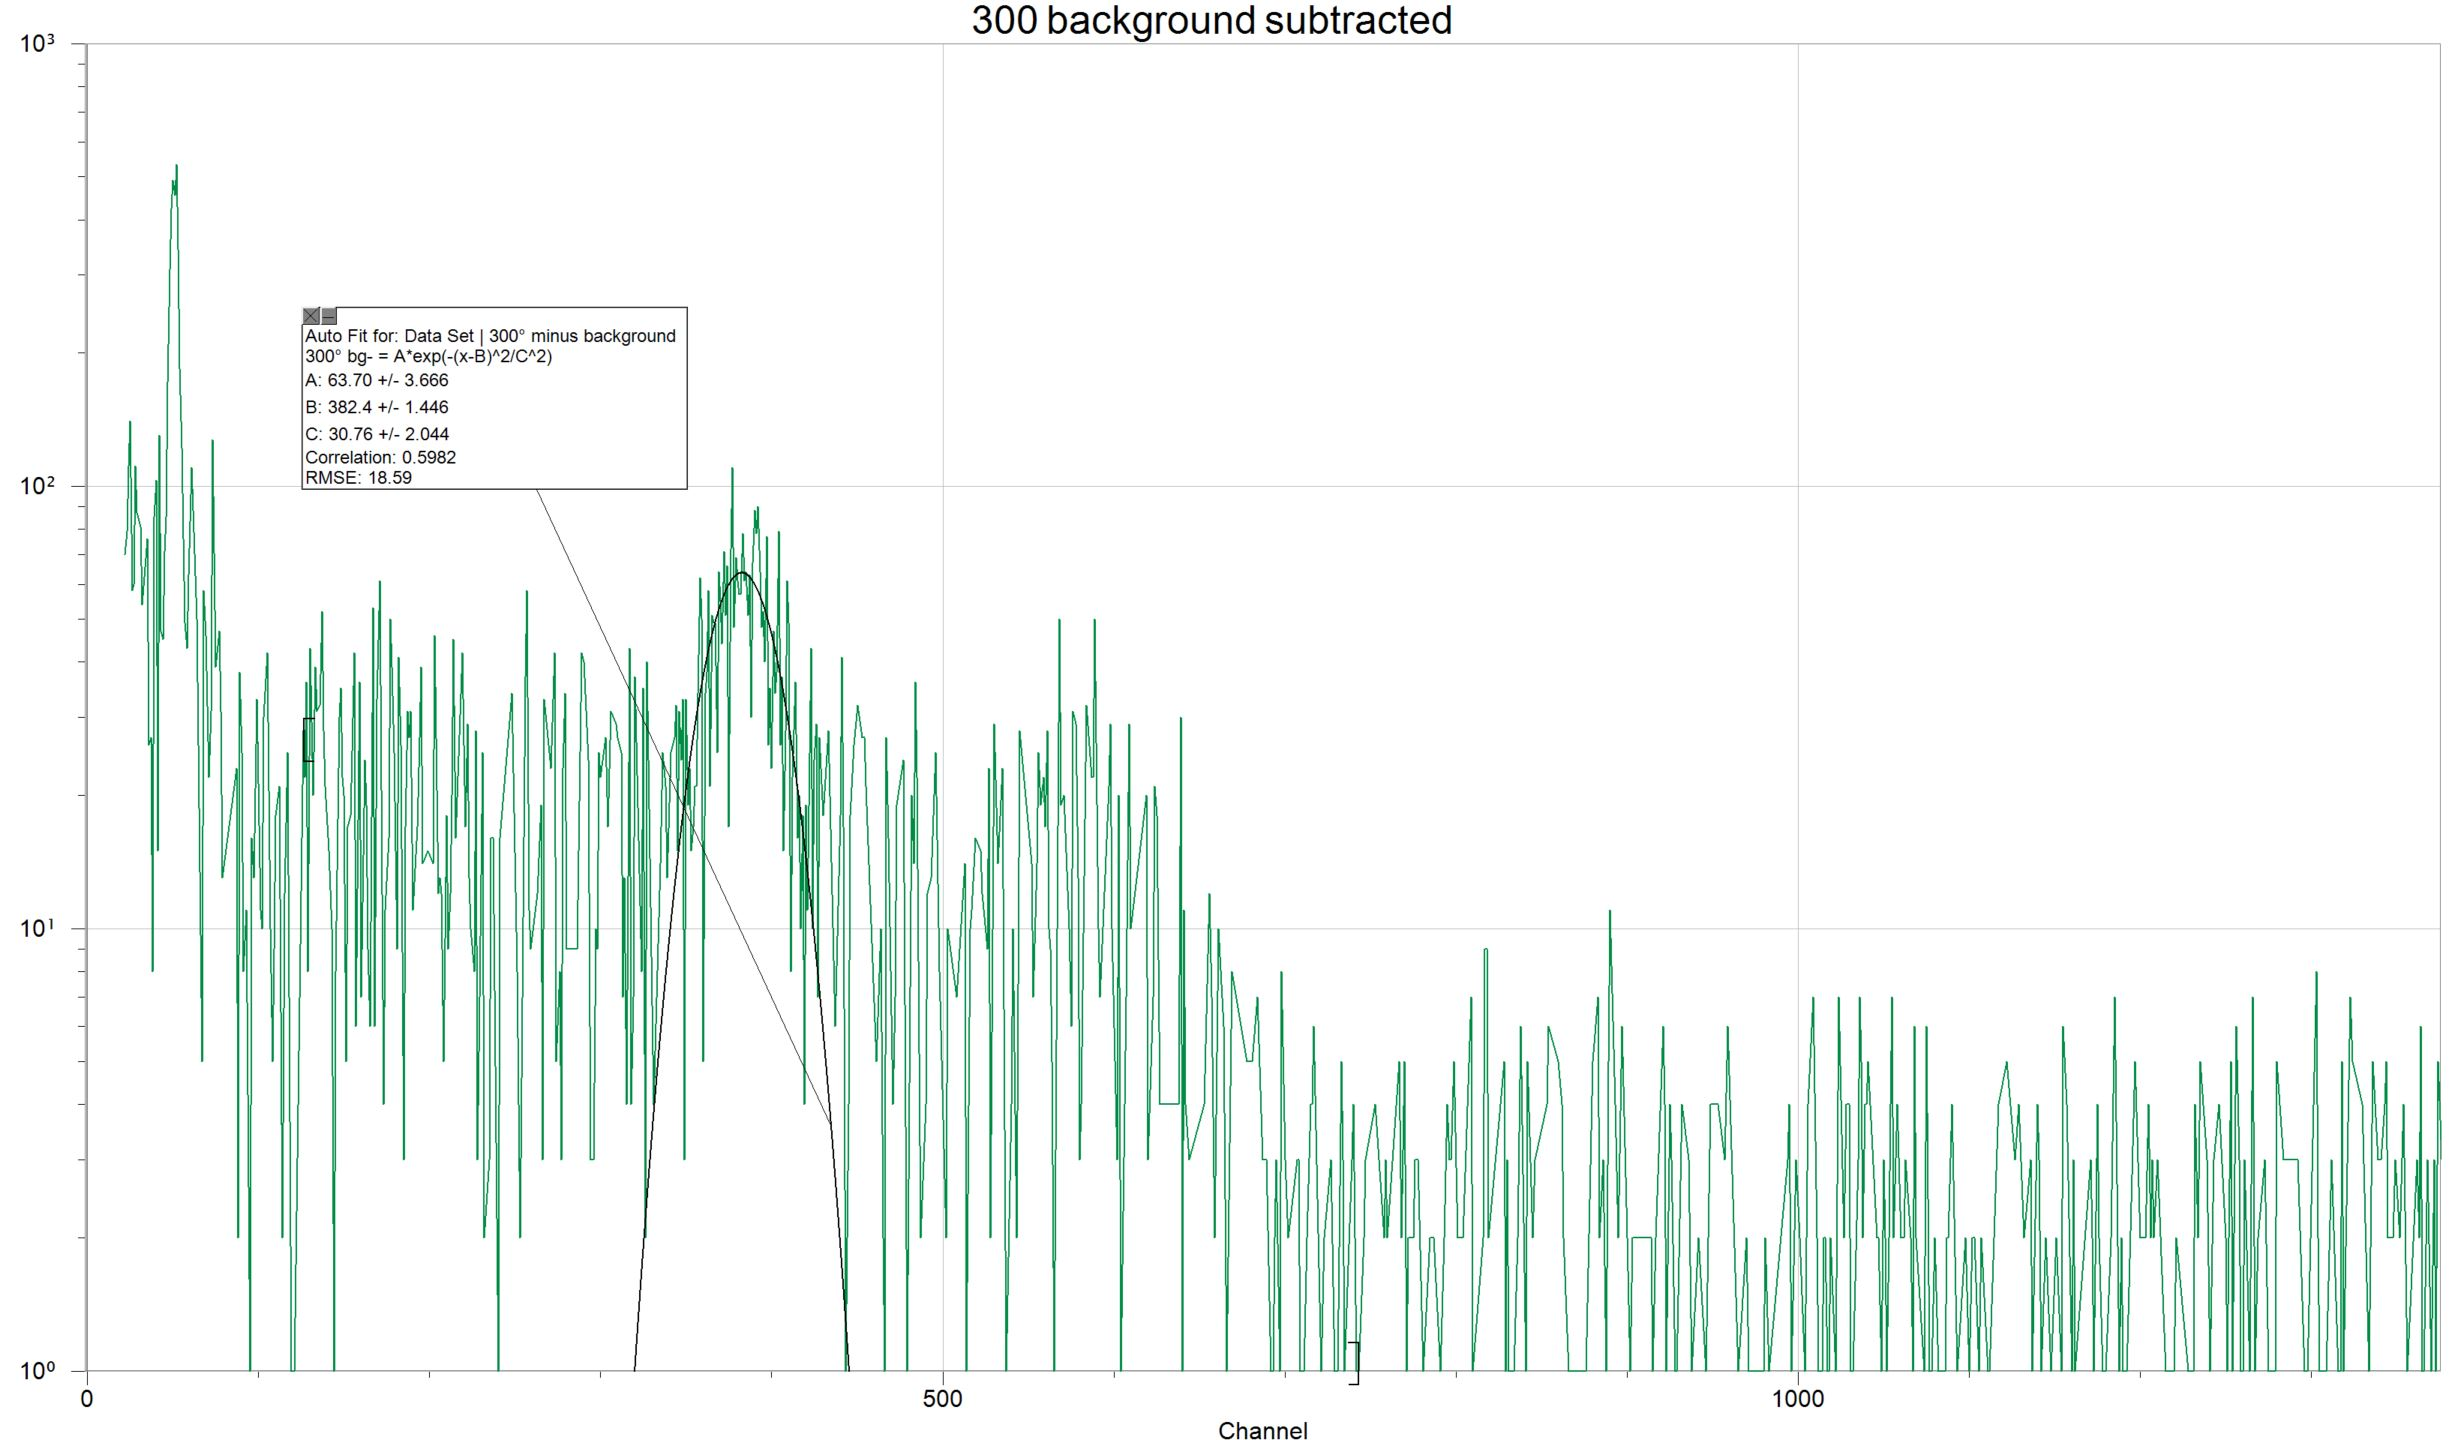
\includegraphics[height=10cm, width=18cm]{Seven.JPG}
    \caption{
      Todo
    }
  \end{figure}

  \pagebreak

  \begin{figure}[htbp]
    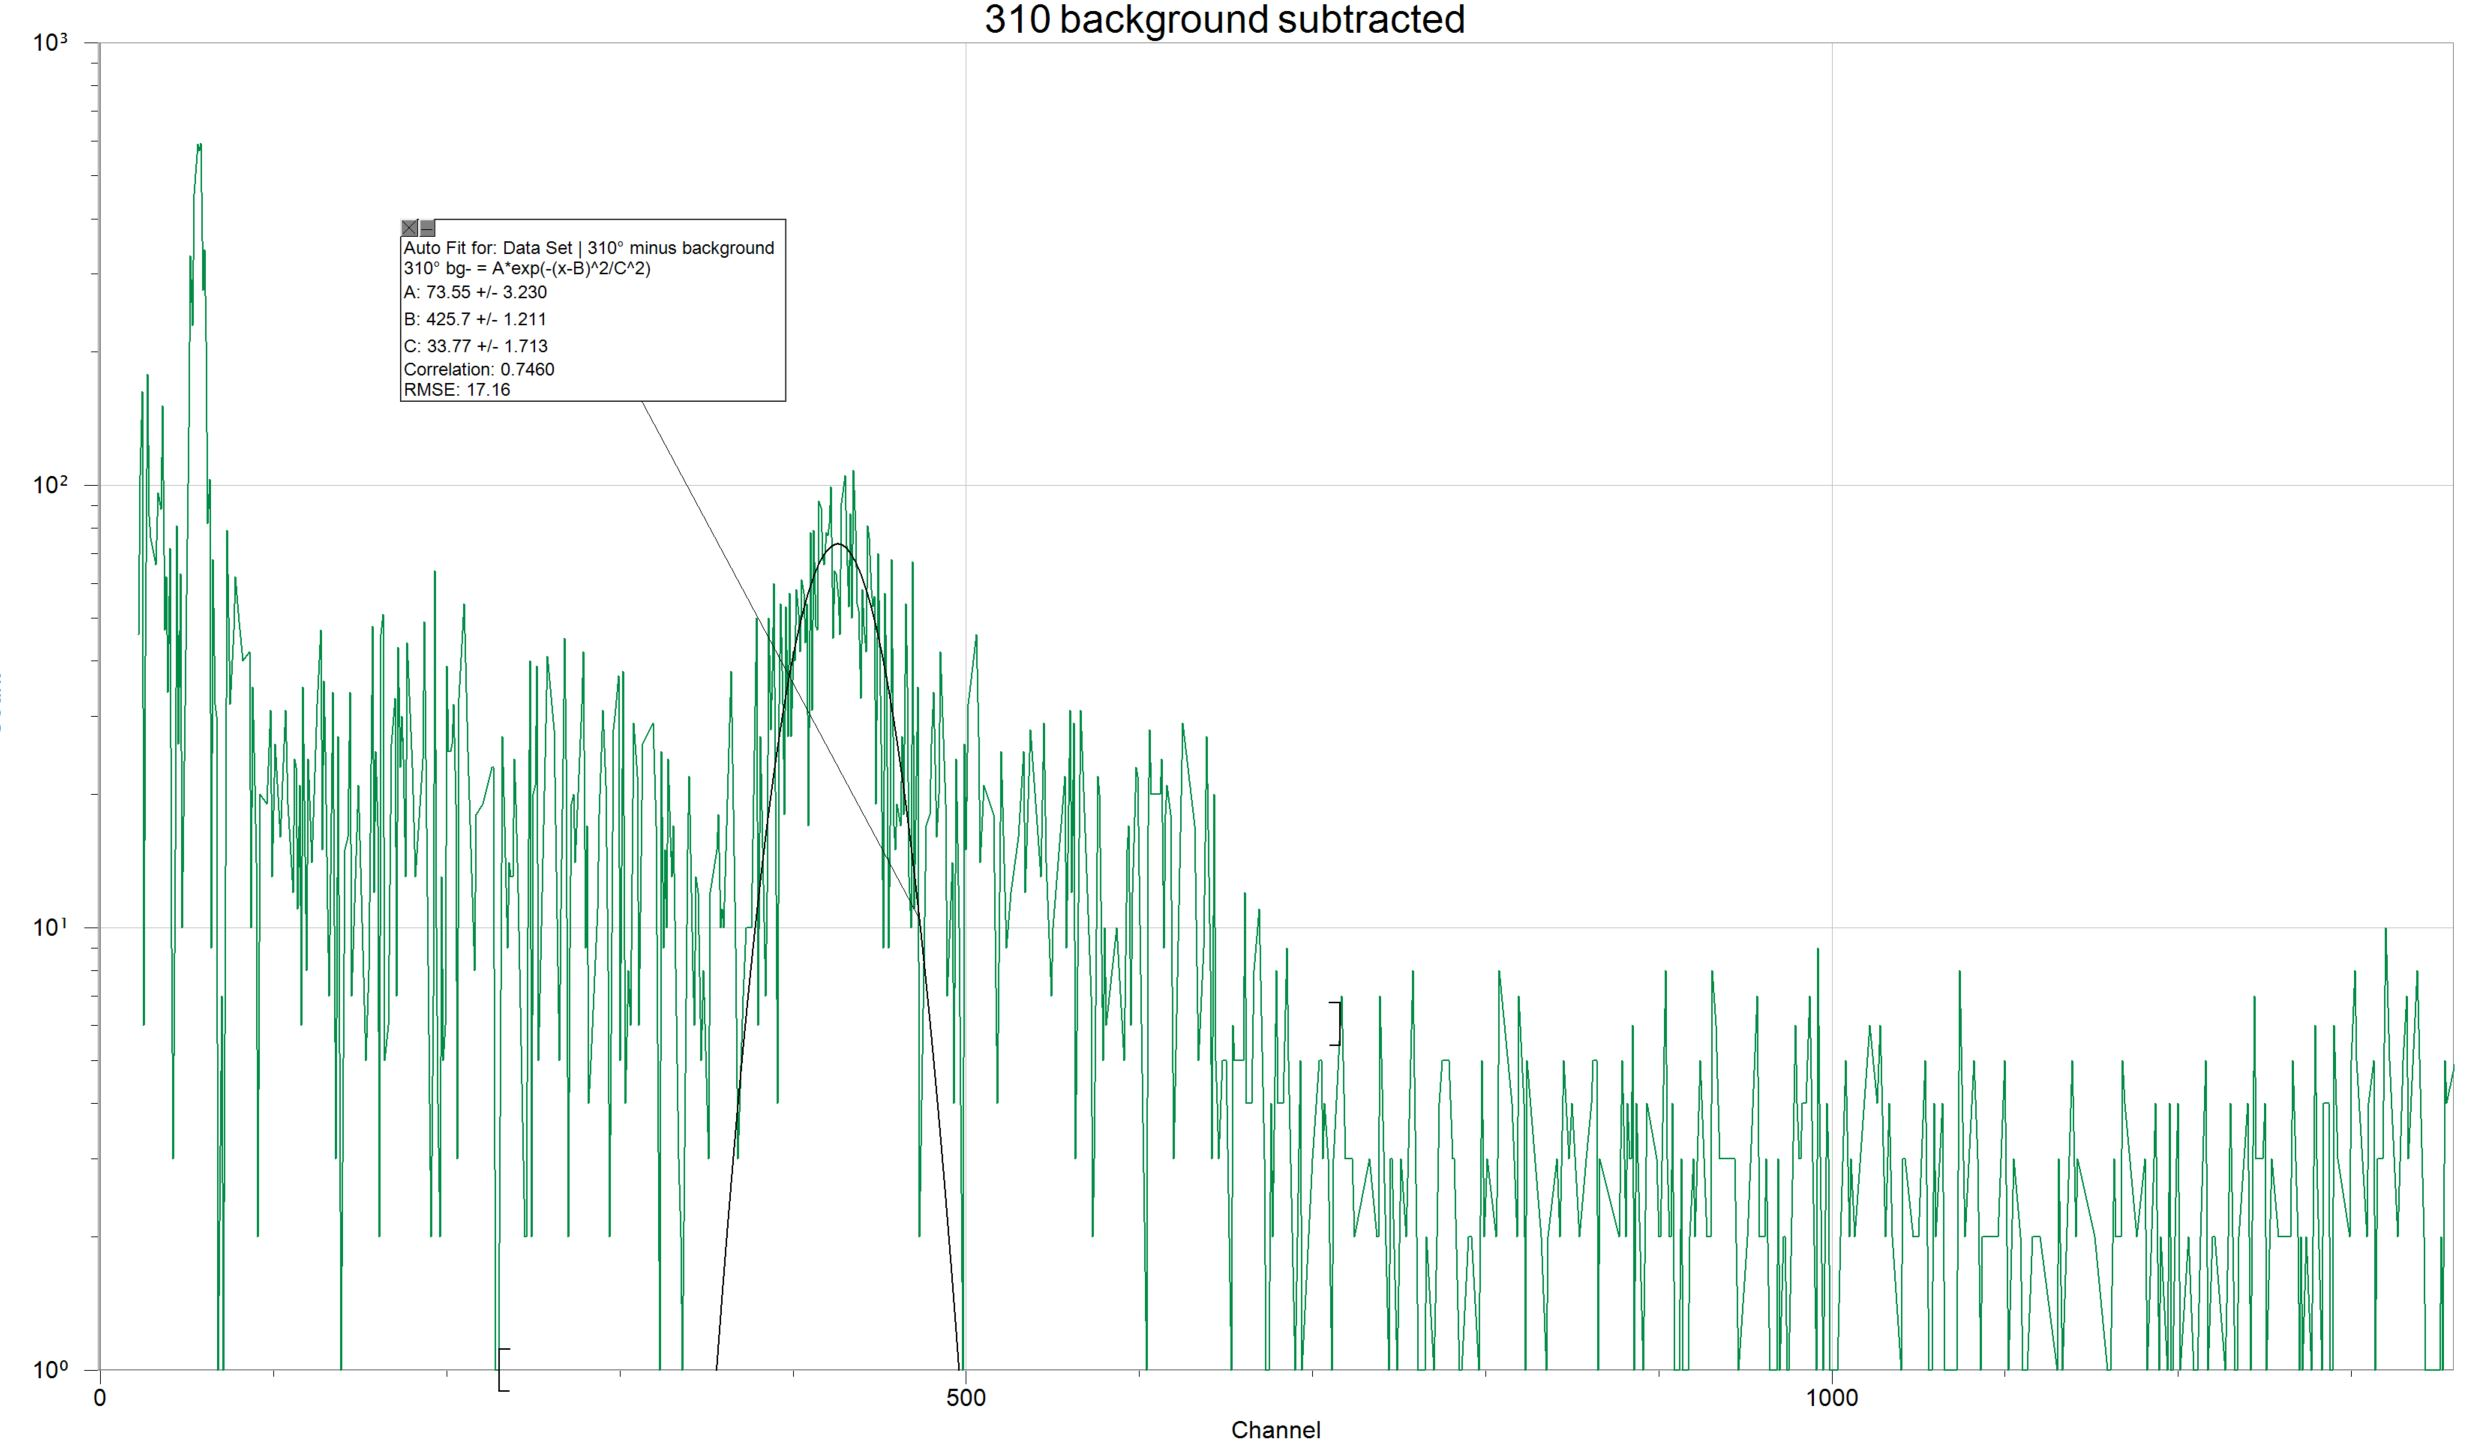
\includegraphics[height=10cm, width=18cm]{Eight.JPG}
    \caption{
      Todo
    }
  \end{figure}

  \pagebreak

  \begin{figure}[htbp]
    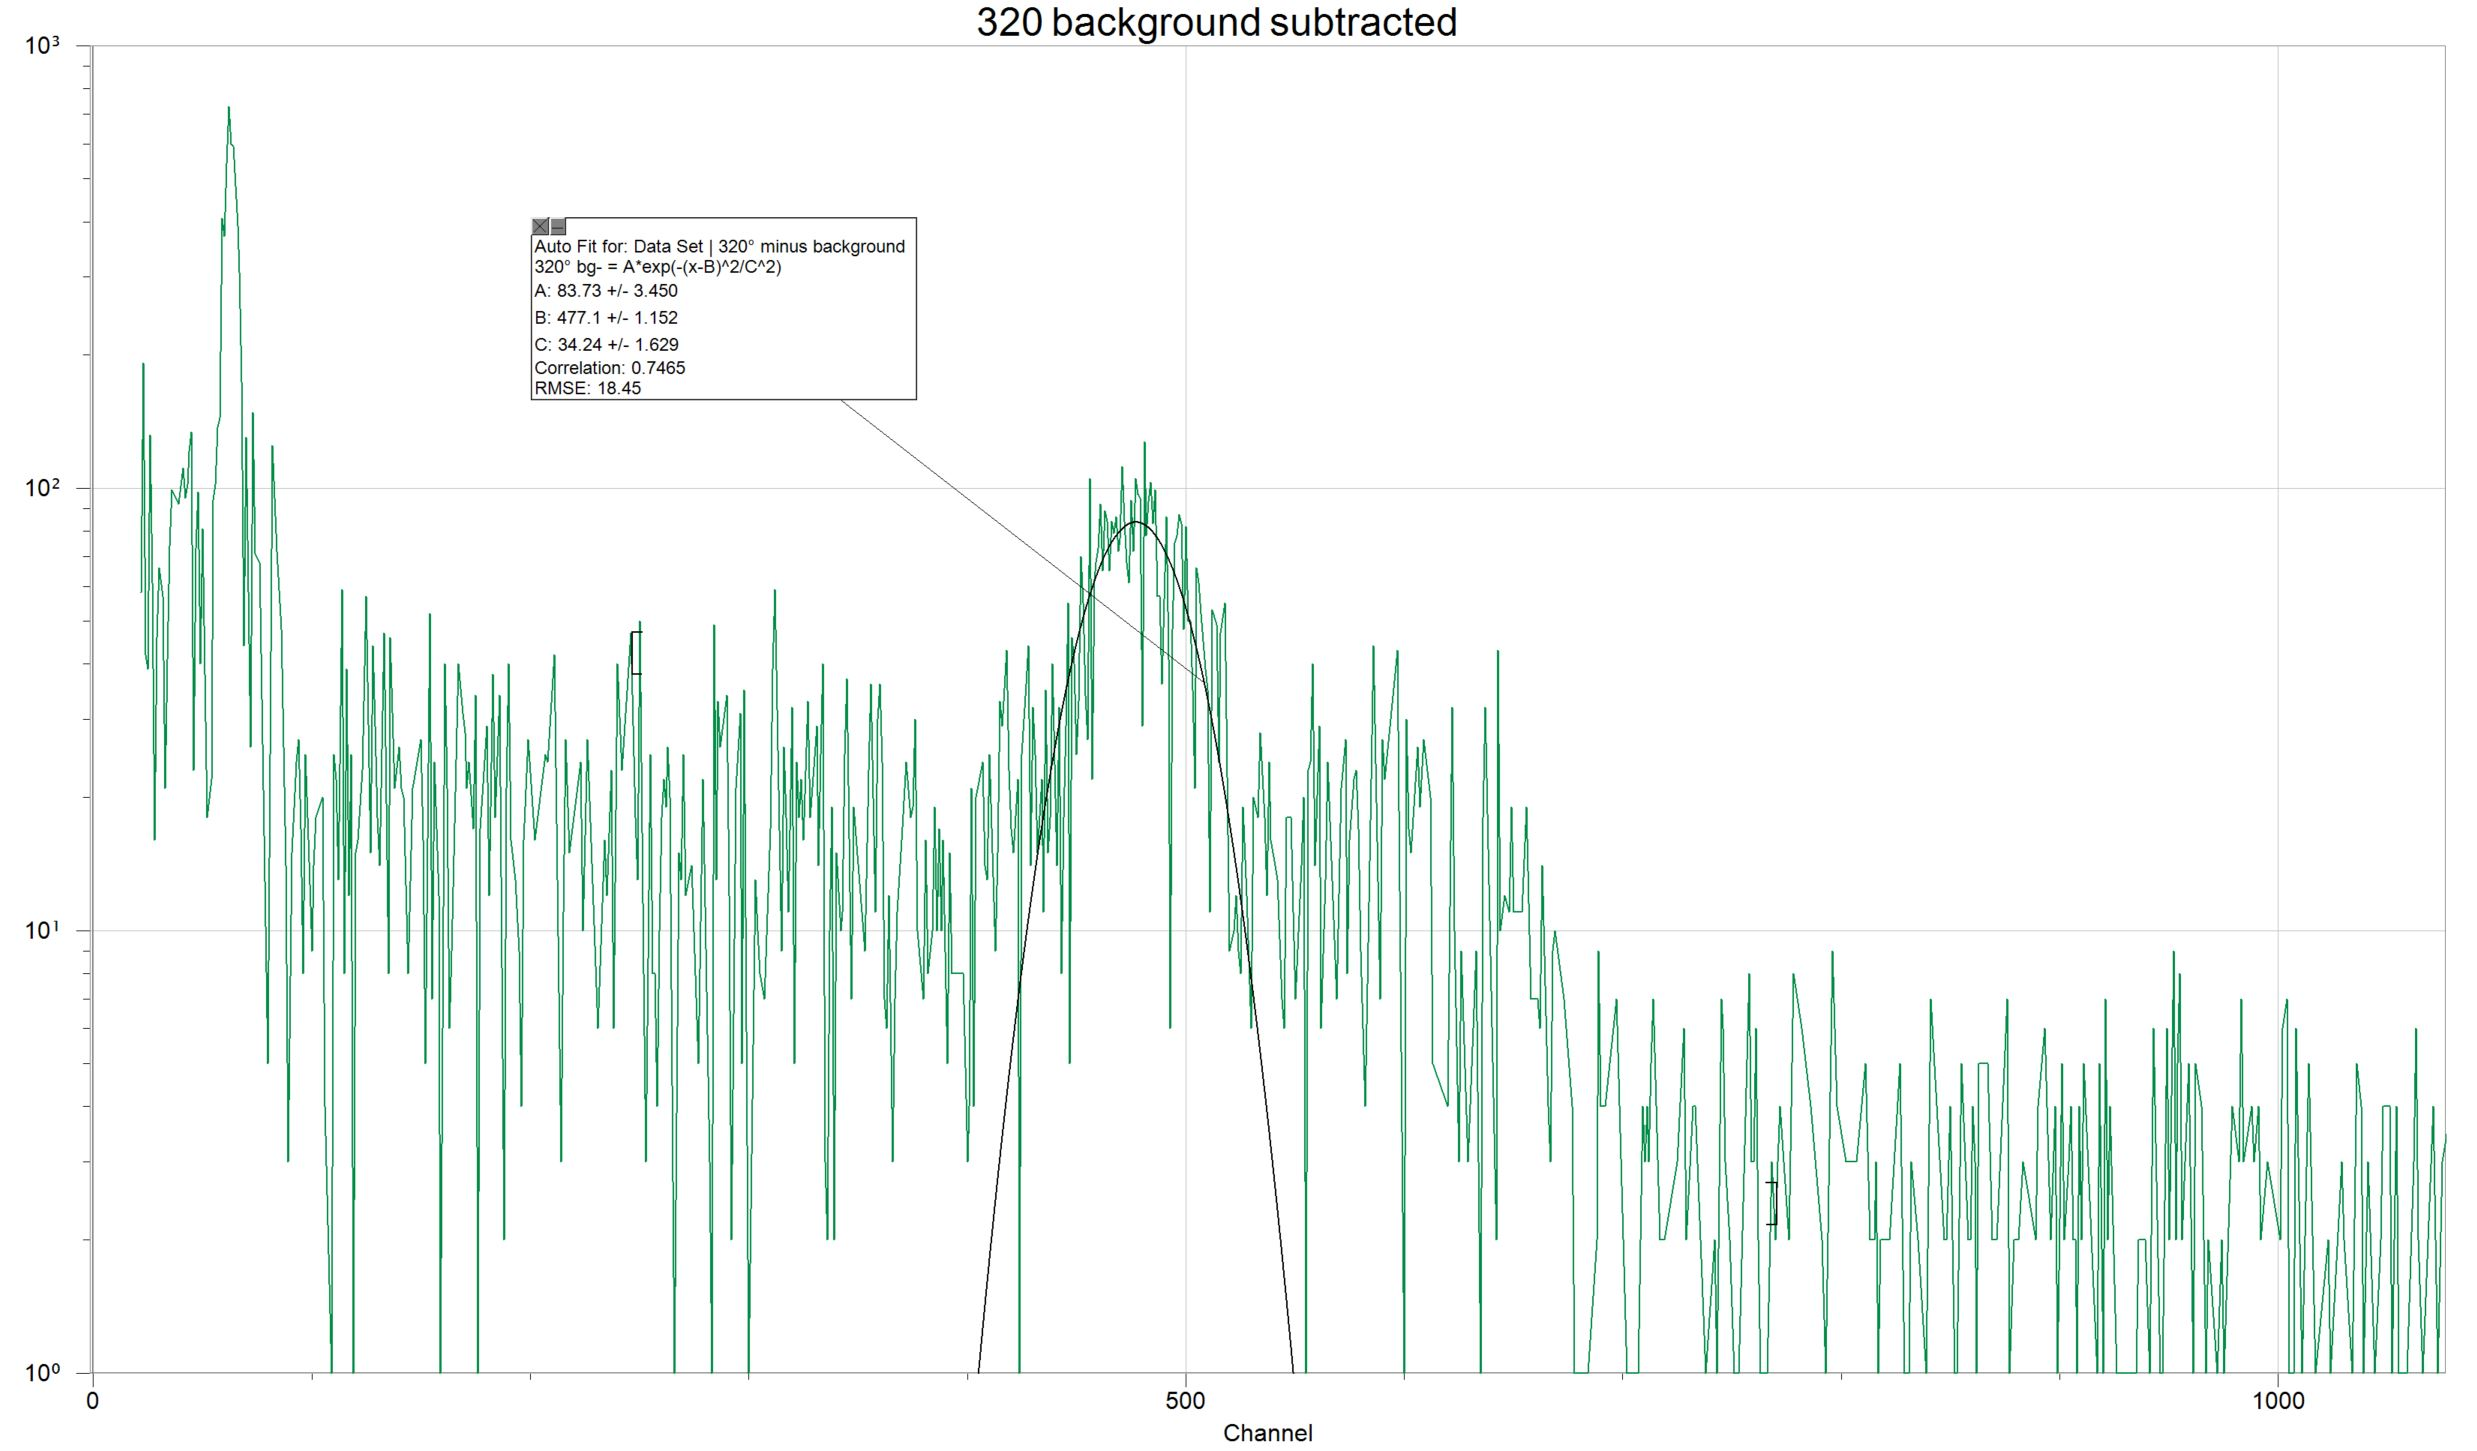
\includegraphics[height=10cm, width=18cm]{Nine.JPG}
    \caption{
      Todo
    }
  \end{figure}

  \pagebreak

  \begin{figure}[htbp]
    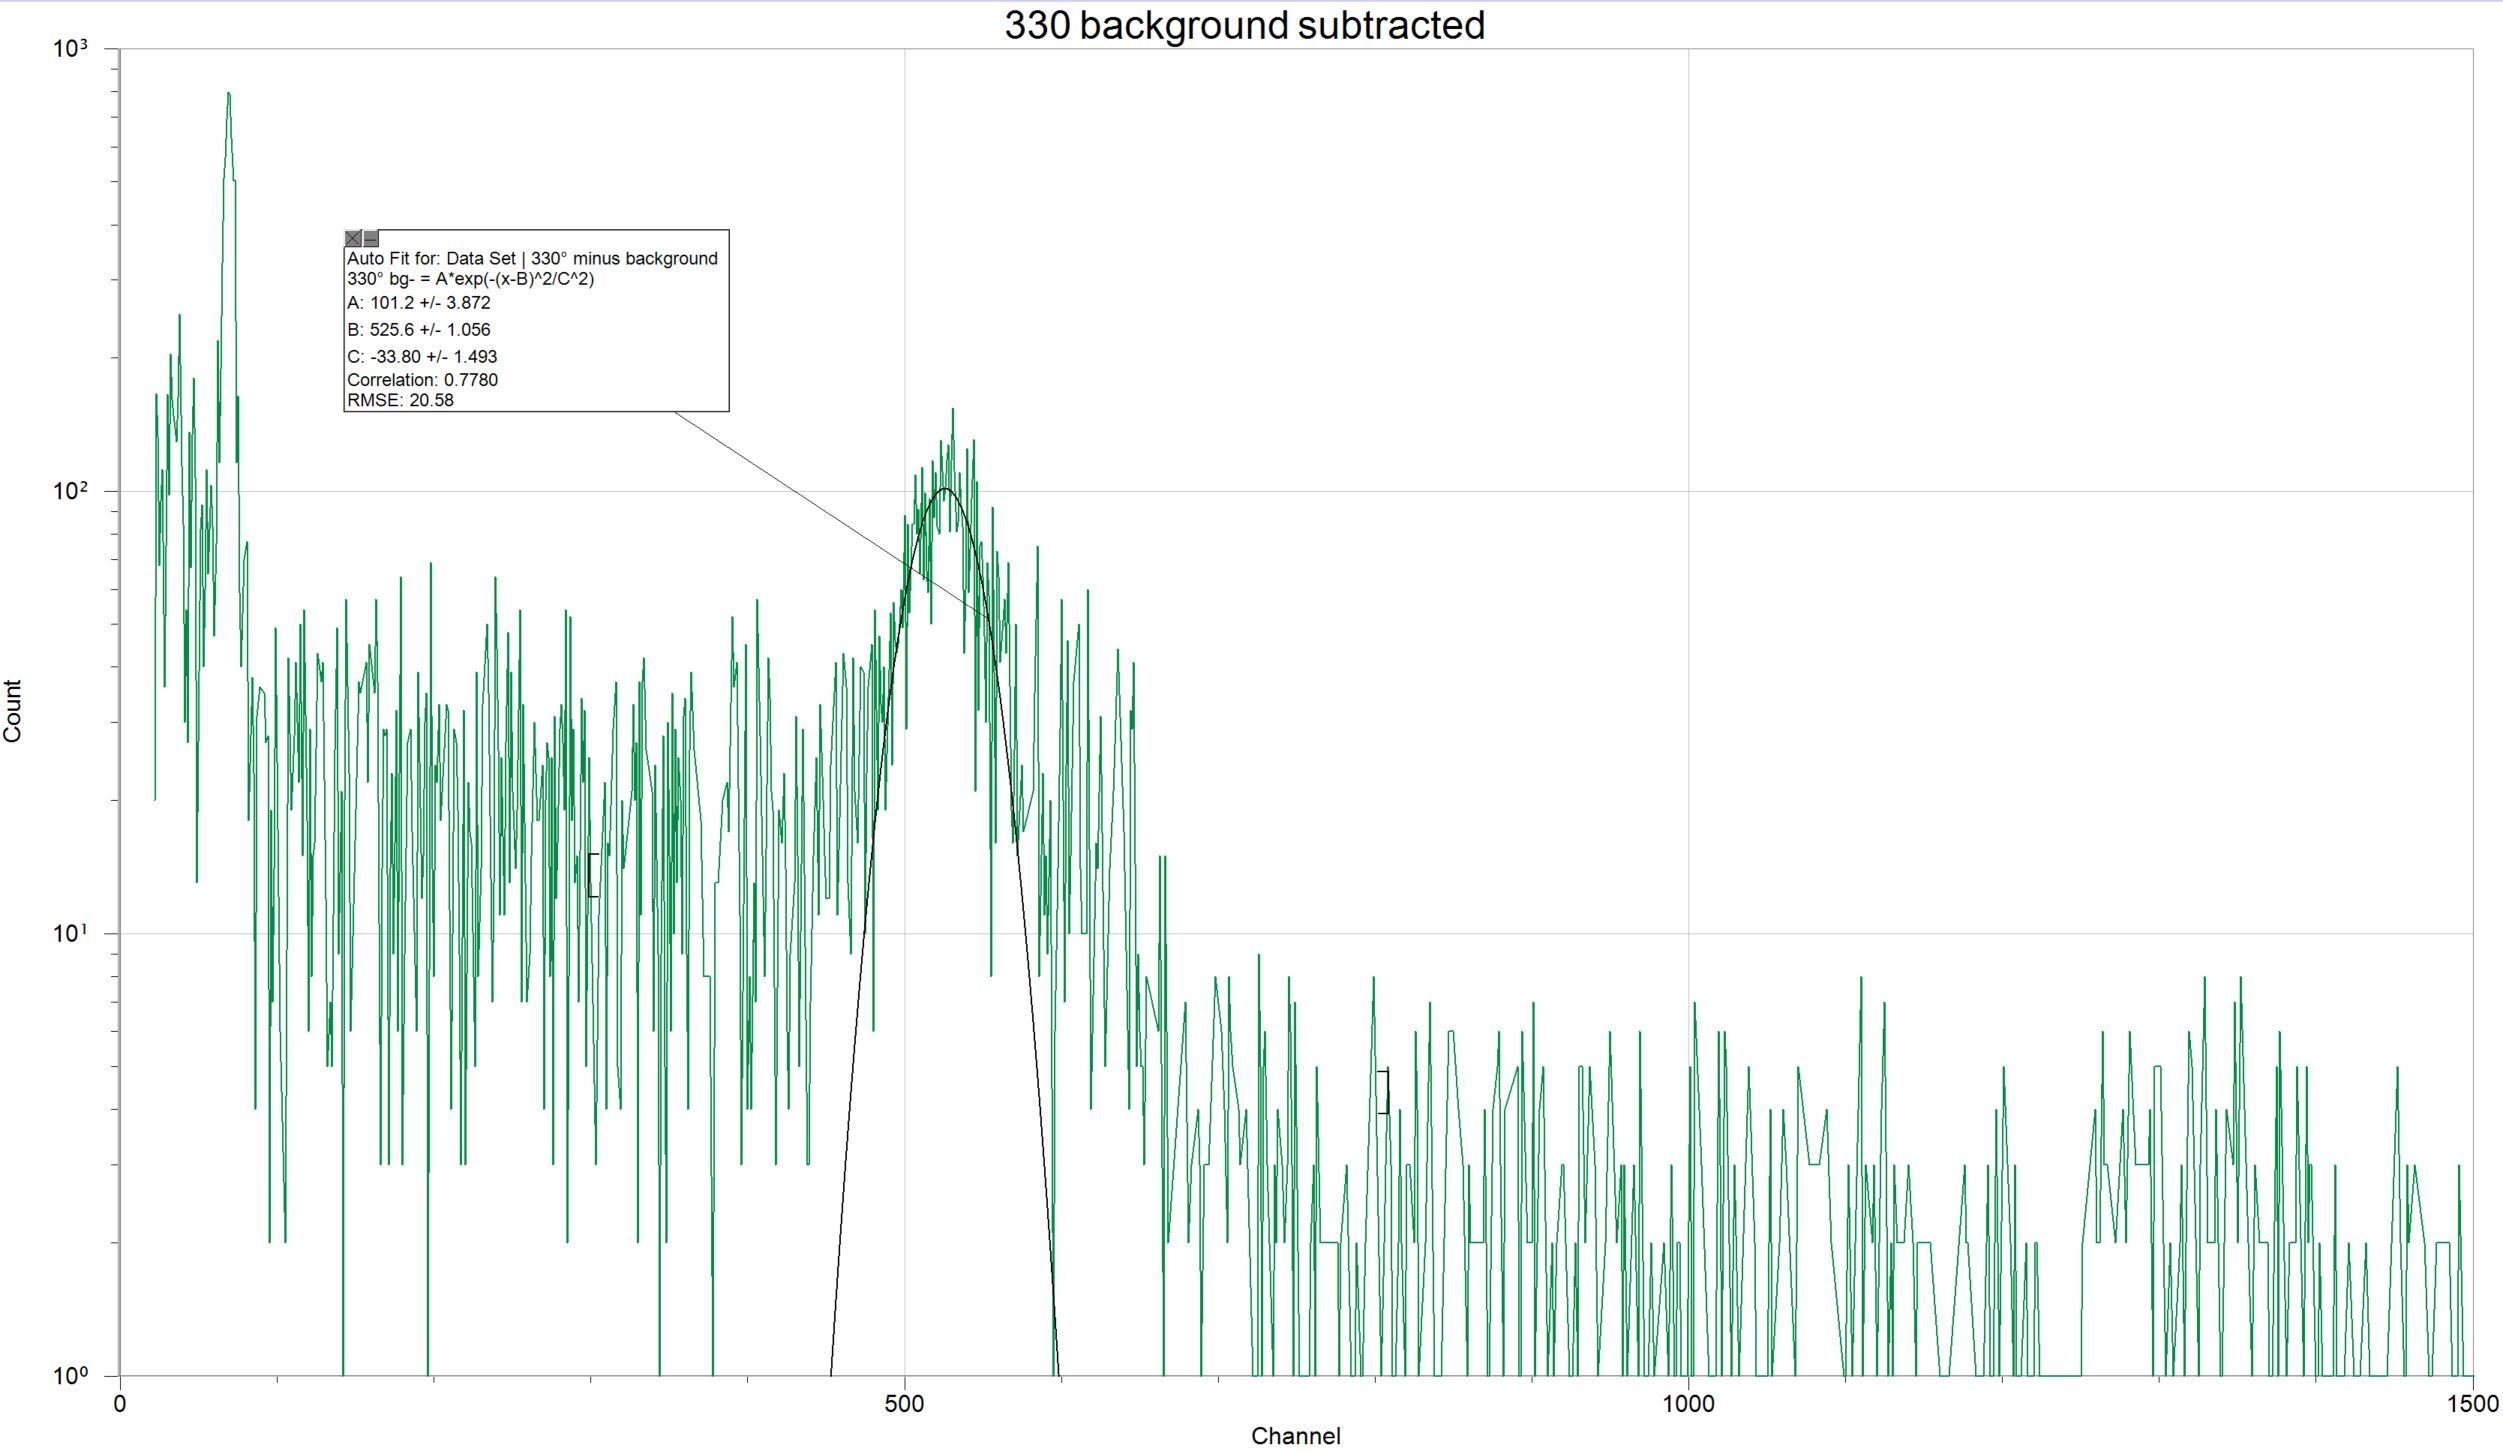
\includegraphics[height=10cm, width=18cm]{Ten.JPG}
    \caption{
      Todo
    }
  \end{figure}

  \pagebreak

  \begin{figure}[htbp]
    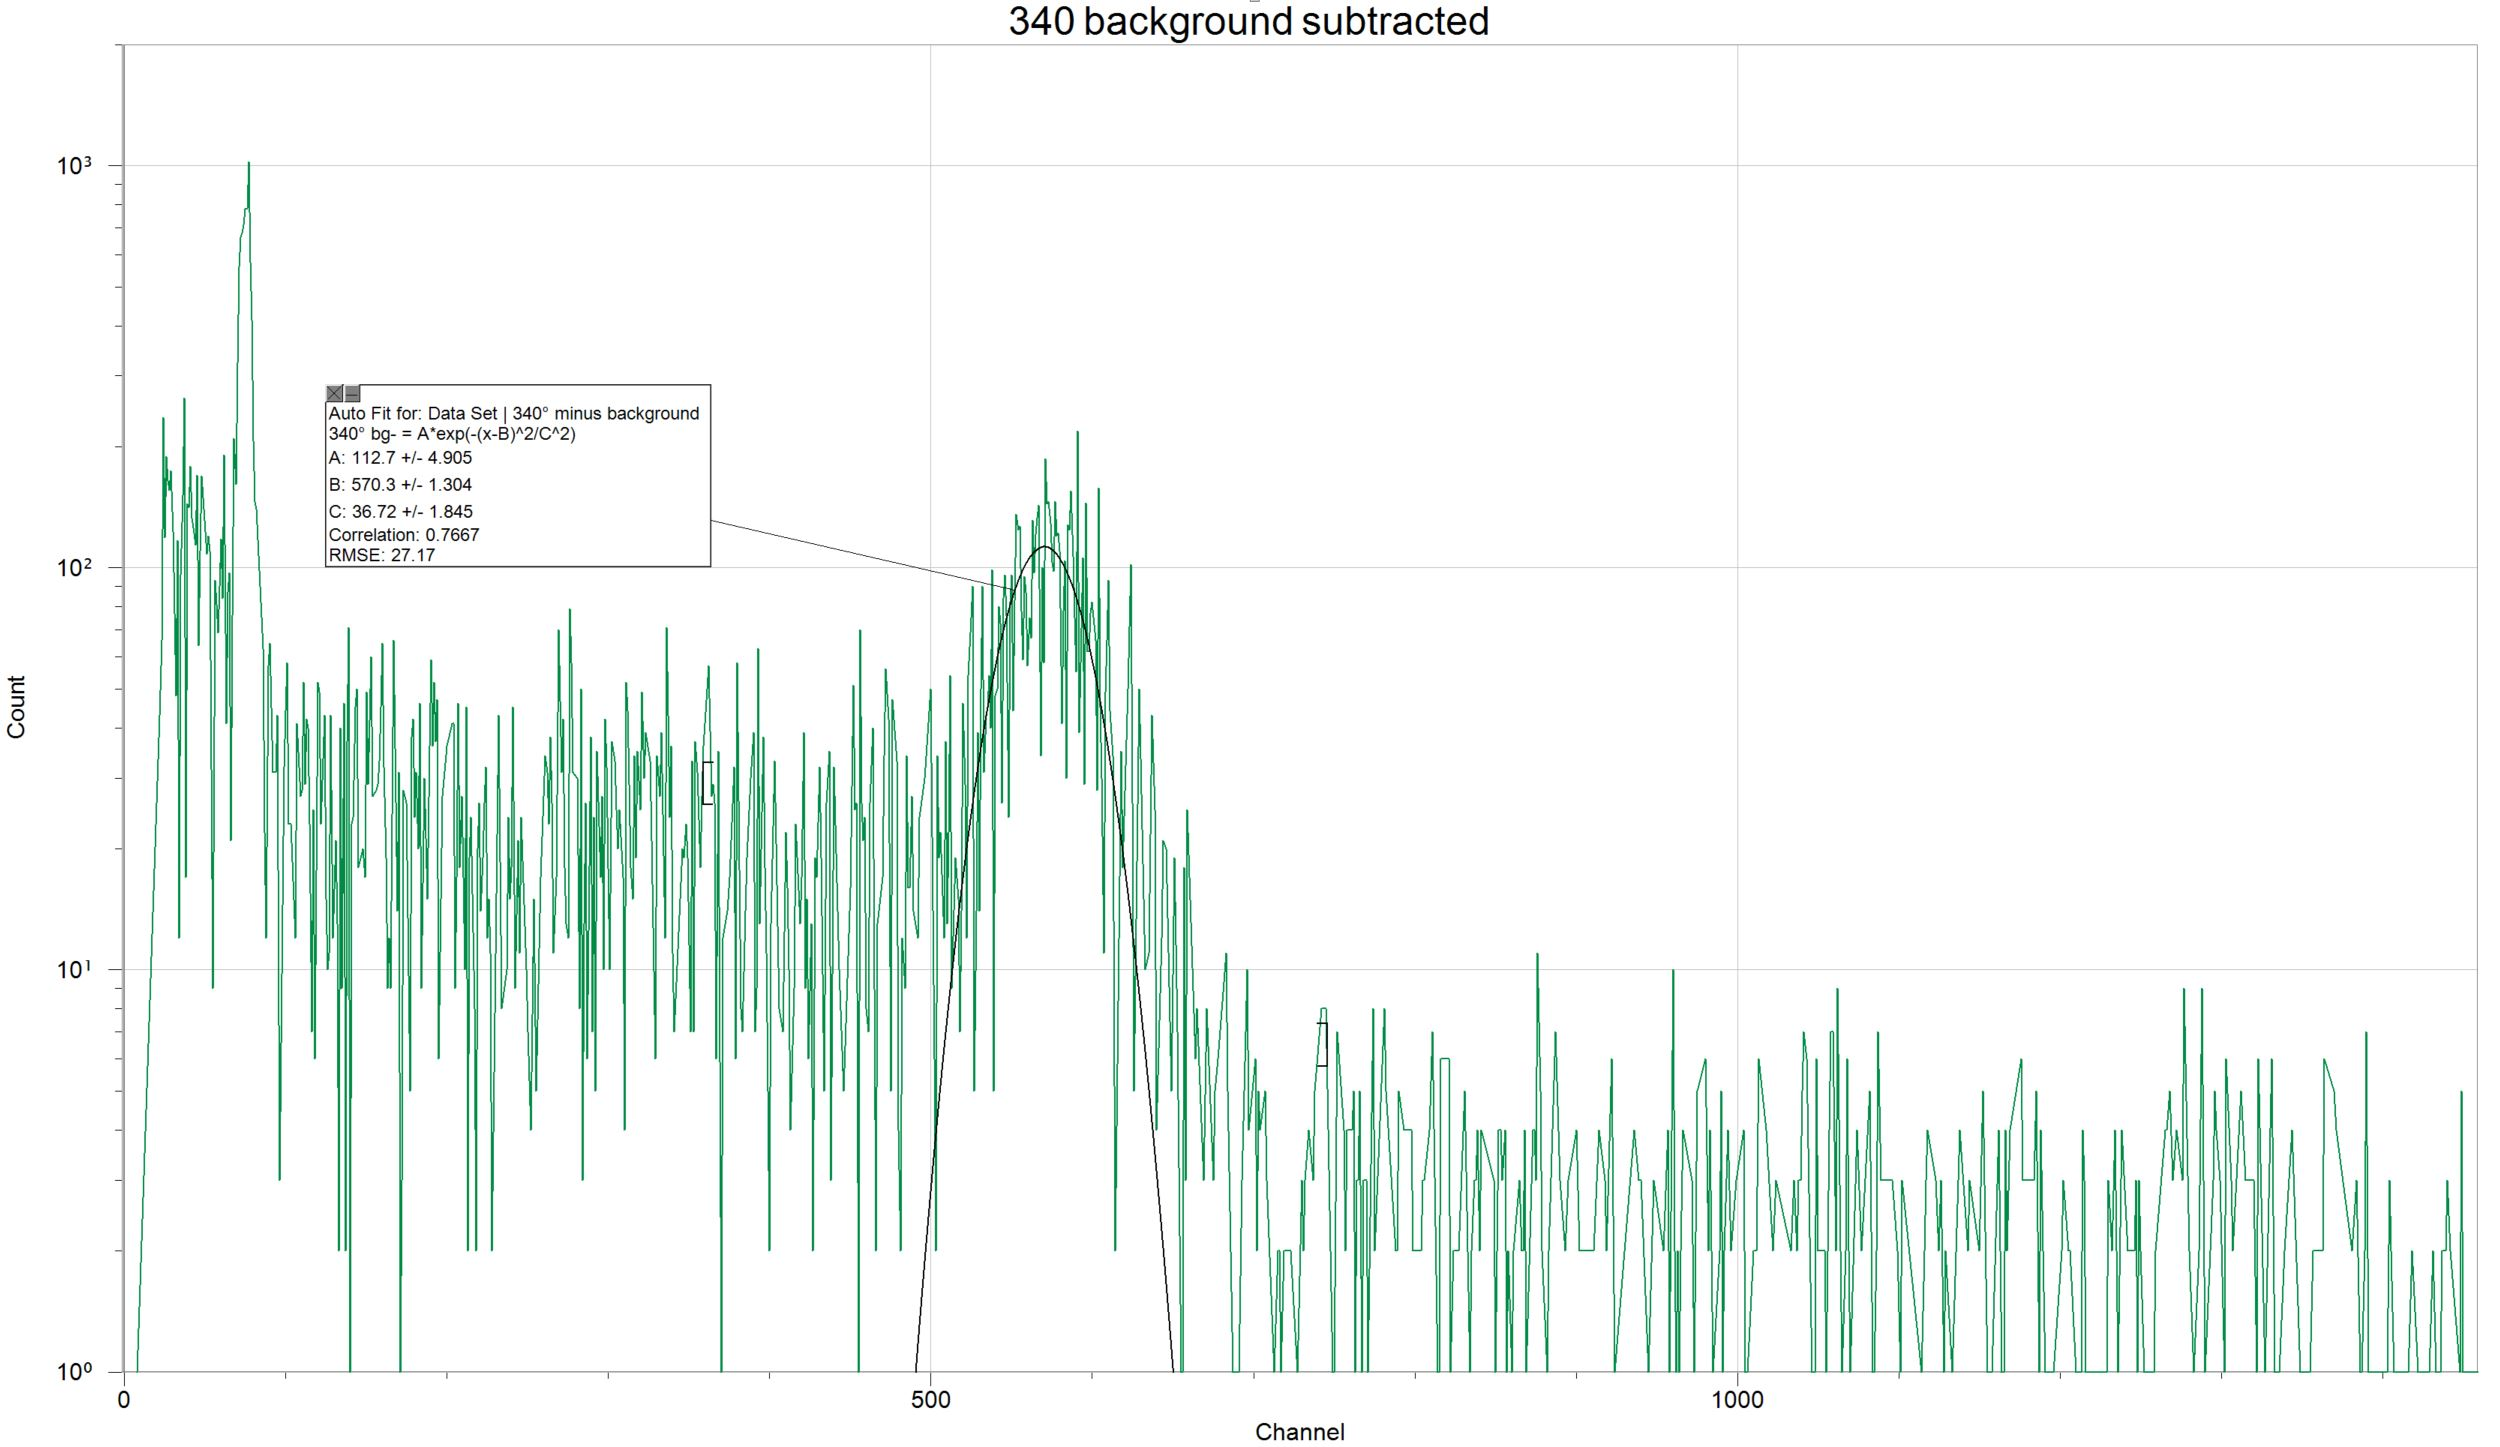
\includegraphics[height=10cm, width=18cm]{Eleven.JPG}
    \caption{
      Todo
    }
  \end{figure}

  \pagebreak

  As it was mentioned in the lab steps we need to rearrange the Compton scattering formula (Eq. 4):
  \\
  \\
  \\
  $
    E^'=\left[1+\left(\dfrac{E}{mc^2}\right)  \left(1-cos(\theta)\right)\right]=E
    \\
    \\
    \\
    \therefore ~~~ E^'=E \left[1+\left(\dfrac{E}{mc^2}\right)  \left(1-cos(\theta)\right)\right]^{-1} ~~~~~~~ (5)
    \\
    \\
  $
  For CS-137 we have $E=662 ~ KeV$ therefore we have
  \\
  \\
  \\
  $
    E^'=E \left[1+\left(\dfrac{662 ~ KeV}{mc^2}\right)  \left(1-cos(\theta)\right)\right]^{-1}
  $
  \\
  \\
  \\
  \\
  By rearranging Eq (5) to form a linear, we get the following
  \\
  \\
  $
    \left(E^'\right)^{-1}=\left(E \left[1+\left(\dfrac{E}{mc^2}\right)  \left(1-cos(\theta)\right)\right]^{-1}\right)^{-1}
    \\
    \\
    \\
    \dfrac{1}{E^'}=\dfrac{1}{E} \left[1+\dfrac{E}{mc^2} \left(1-cos(\theta)\right)\right]
    \\
    \\
    \\
    \dfrac{1}{E^'}=\dfrac{1}{E}+\dfrac{1}{mc^2} \left(1-cos(\theta)\right)
    \\
    \\
    \\
    \dfrac{1}{E^'}=\left(\dfrac{1}{E}+\dfrac{1}{mc^2}\right)-\dfrac{1}{mc^2} cos(\theta)
    \\
    \\
    \\
    \\
    \begin{cases}
      y=\dfrac{1}{E^'}
      \\
      \\
      \alpha=\dfrac{1}{E}+\dfrac{1}{mc^2}
      \\
      \\
      \beta=-\dfrac{1}{mc^2}
      \\
      \\
      x=cos(\theta)
    \end{cases}
    \Longrightarrow
    y=\beta x+\alpha
    \\
    \\
    \\
    \\
    \begin{cases}
      \alpha=\dfrac{1}{\left(662 \times 10^3 ~ eV\right) \left(1.6021 \times 10^{-19}\right)}+\dfrac{1}{\left(9.11 \times 10^{-31} ~ kg\right) ~ \left(3 \times 10^8 ~ m/s\right)^2}=2.1625 \times 10^{13} ~~ J^{-1}
      \\
      \\
      \beta=-\dfrac{1}{9.11 \times 10^{-31} ~ kg \left(3 \times 10^8 ~ m/s\right)^2}=-1.2197 \times 10^{13} ~~ J^{-1} 
    \end{cases}
    \\
    \\
    \\
    \\
    \\
    \therefore ~~~~ y=-\left(1.2197 \times 10^{13}\right) x+\left(2.1625 \times 10^{13}\right) ~~~ \checkmark
    \\
    \\
    \\
    \\
    \therefore ~~~~ E^'=\dfrac{1}{-\left(1.2197 \times 10^{13}\right) x+\left(2.1625 \times 10^{13}\right)} ~~~ \checkmark
    \\
    \\
    \\
  $
  Now based on the obtained equations we have the experimental electron masss as
  \\
  \\
  \\
  $
    m=2\dfrac{1}{c^2 \left(\alpha-\beta-\dfrac{1}{E}\right)}
    =2\dfrac{1}{\left(3 \times 10^8\right)^2 \left(
      \left(2.1625 \times 10^{13}\right)
      +\left(1.2197 \times 10^{13}\right)
      -\dfrac{1}{662 \times 10^3}
    \right)}
    \\
    \\
    \\
    \\
    \therefore ~~~~ m=6.66 \times 10^{-31} ~~~ kg
  $

  TODO Peak Energy goes here

  \pagebreak

  \textbf{VI. Discussion}

  \pagebreak

  \textbf{VII. Conclusions}

  \vspace{10px}

  The main aims of this experiment were to provide experimental evidence of the Compton Effect by showing that the model of the Compton Effect,
  Eq. (3), fitted with the experimental data. By providing such evidence, an experimental value of the electron mass m was obtained.

  \pagebreak

  \textbf{VIII. References}

  \vspace{15px}

  Rae, A.I. (2008). Quantum Mechanics (5th ed.). Taylor and Francis Group.

  \vspace{5px}

  8.13-14 Experimental Physics I \& II "Junior Lab" Fall 2016 - Spring 2017.

\end{document}
